\section{Gjennomføring med måleresultater}
    I dette kapittelet presenteres resultatene fra de forskjellige kretsene det er gjort målinger på. Resultatene presenteres i form av bilder tatt direkte av oscilloskopet og signalene som vises der. Hensikten er å vise hvordan oppgaven utføres i praksis og hvordan de resultatene man får oppstår. 
    \subsection{Måling på enkel klippekrets}
        Den første kretsen som skal gjennomføres måling på er en enkel klippekrets illustrert i figur \ref{fig:enkel_klippekrets1}.
        Kretsen ble koblet eksakt som det er illustrert i figuren, og oscilloskopet brukes deretter til å sammenligne den teoretiske kurven for spenningen over dioden med de målte spenningskurvene på oscilloskopet.
        \begin{figure}[H]
            \centering
            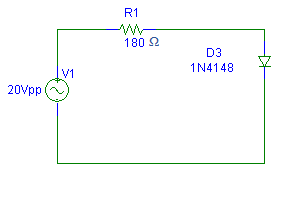
\includegraphics[width=0.7\textwidth]{Media/klippekrets.png}
            \caption{Enkel klippekrets}
            \label{fig:enkel_klippekrets1}
        \end{figure}

        Fra figur \ref{fig:enkel_klippekrets2} ser man en blå og en gul kurve i oscilloskopet. Disse representerer spenningen fra henholdsvis $V1$ og over dioden $D3$. 
        Figuren bekrefter den teoretiske kurven illustrert i figur \ref{fig:python_enkel_klippekrets}. Spenningen over $D3$ klippes på omtrent $0.7V$ i positiv halvperiode, og i negativ halvperiode er spenningen over $D3$ omtrent lik inngangsspenningen.

        \begin{figure}[H]
            \centering
            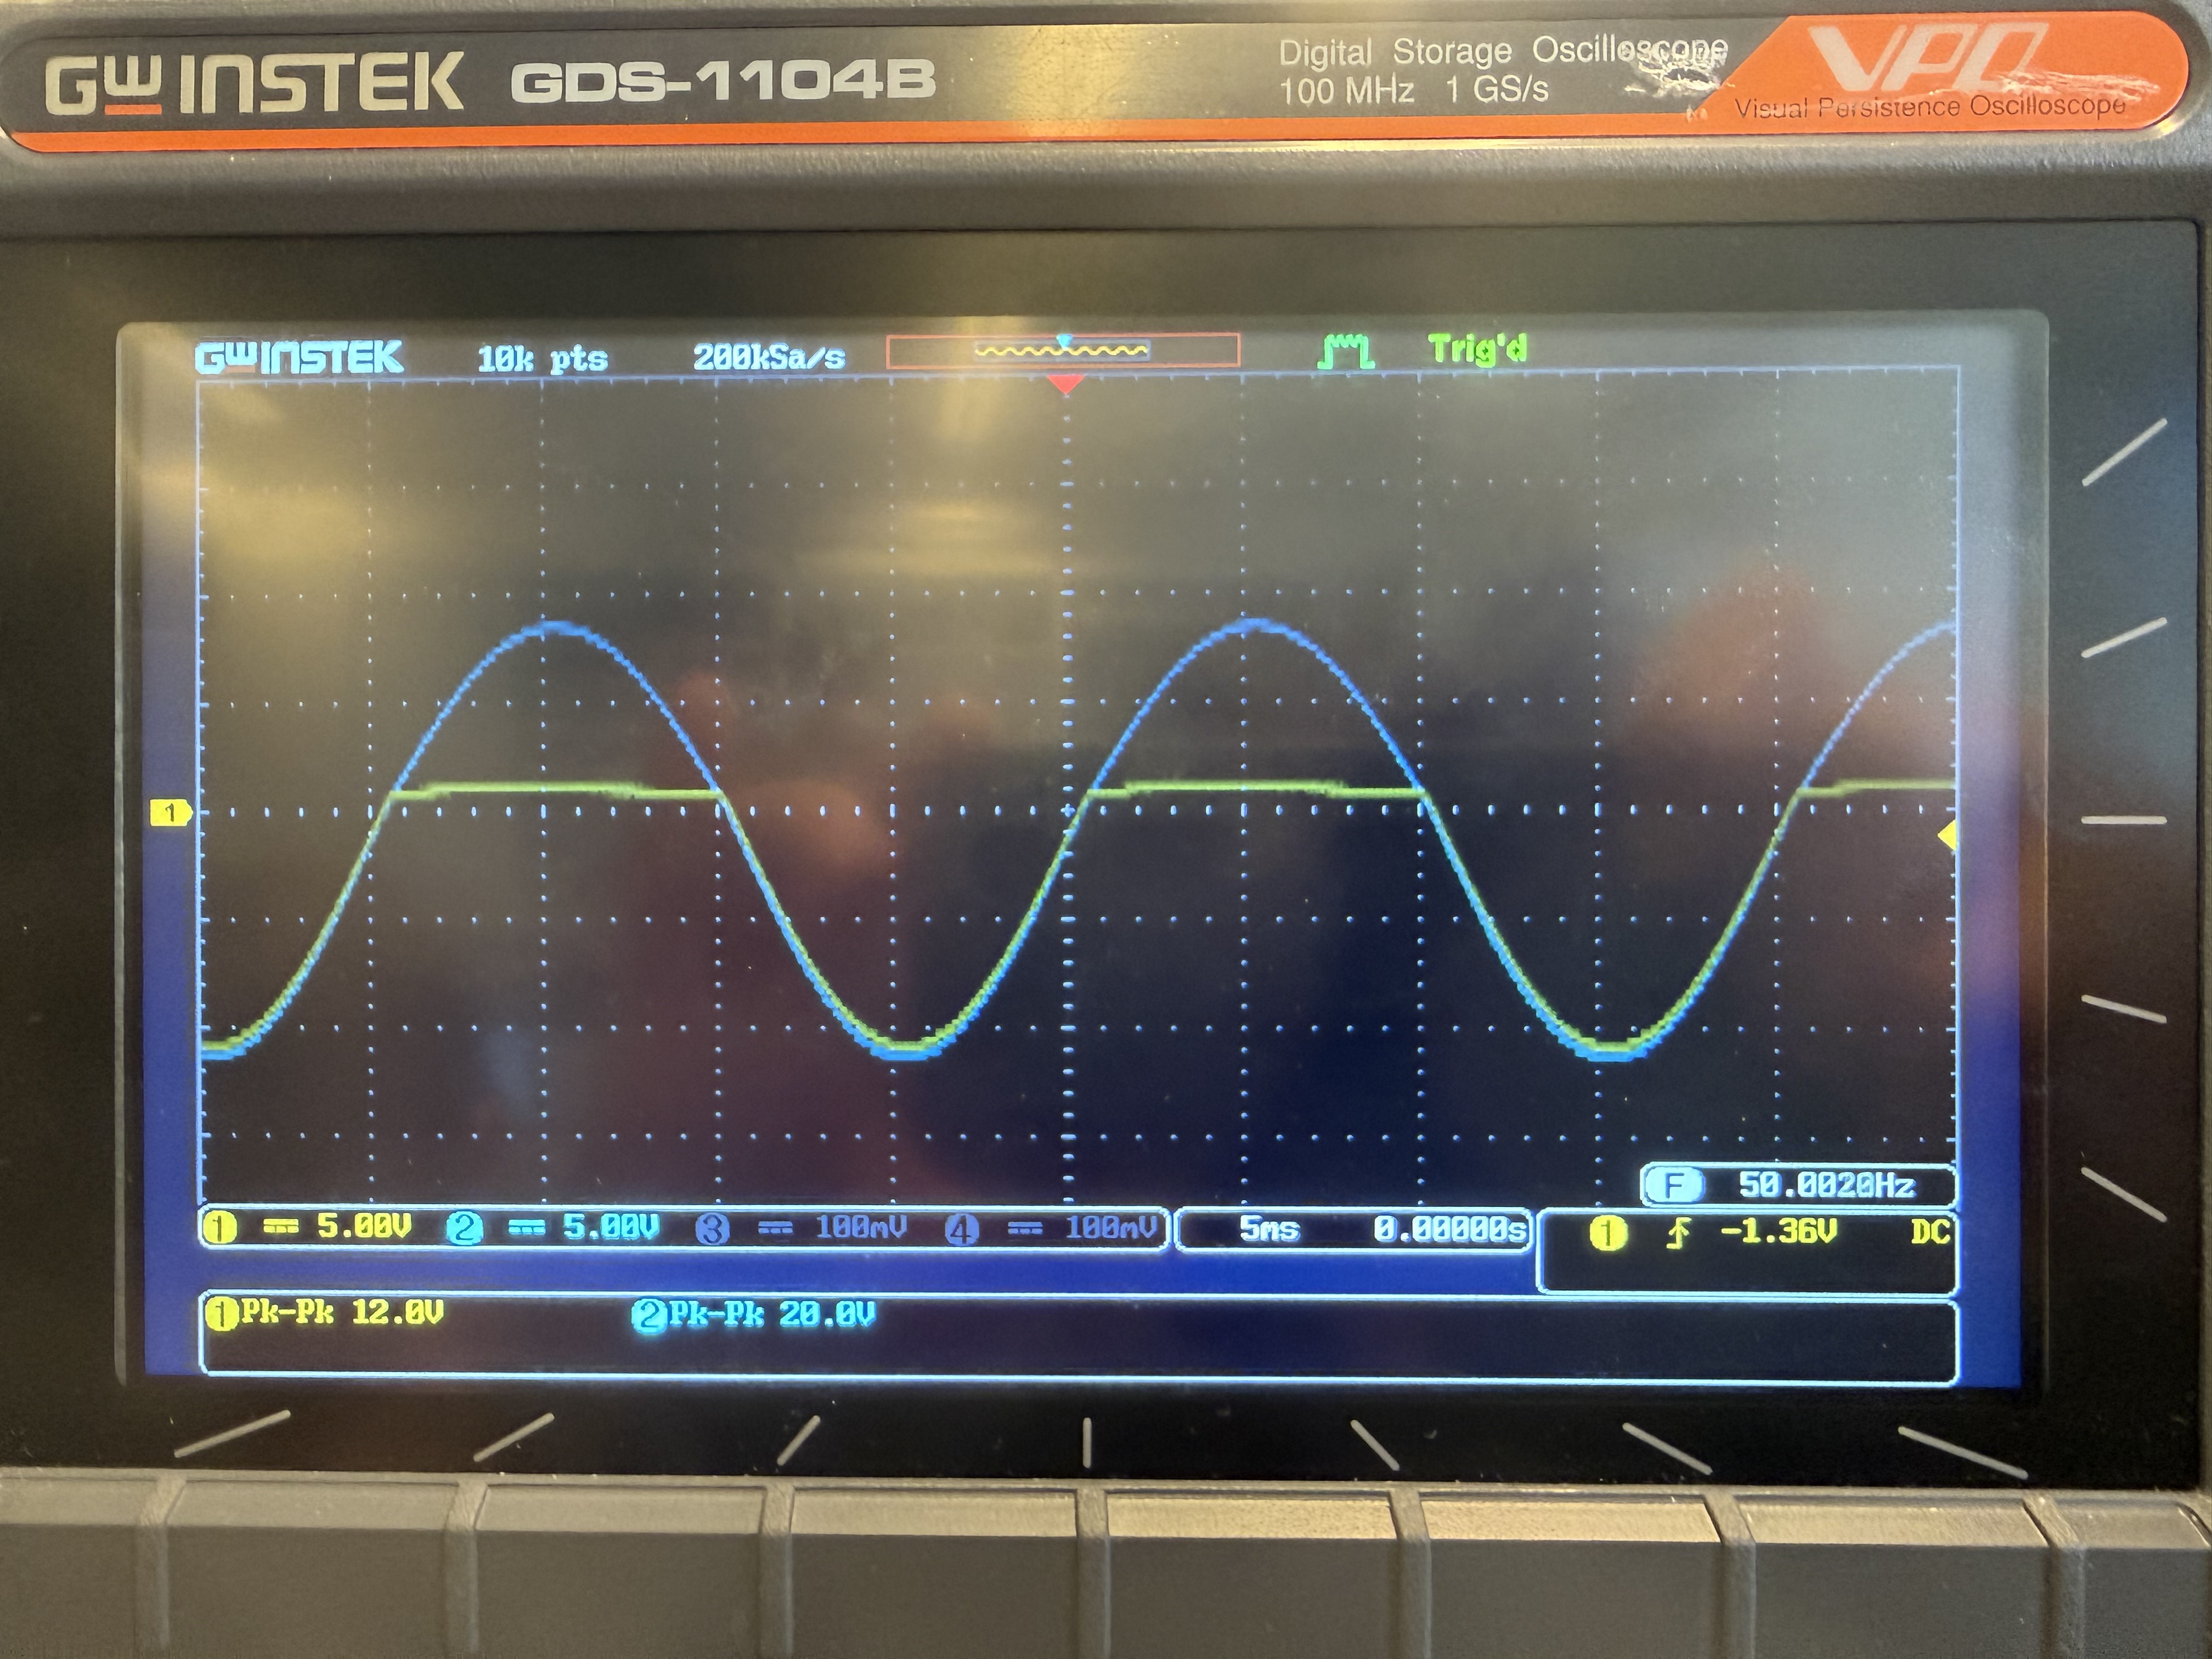
\includegraphics[width=0.7\textwidth]{Media/IMG_0866.jpeg}
            \caption{Måling på enkel klippekrets}
            \label{fig:enkel_klippekrets2}
        \end{figure}

    \subsection{Måling på utvidet klippekrets}
        Videre kobles en diode $D5$ til i parallell med $D3$. Kretsen er koblet eksakt som illustrert i figur \ref{fig:utvidet_klippekrets1}. 
        Igjen så er hensikten å sammenligne den teoretiske kurven med de faktiske faktiske spenningskurvene.
        \begin{figure}[H]
            \centering
            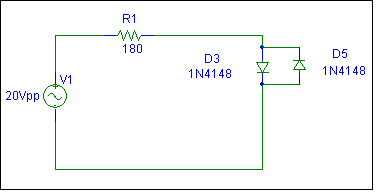
\includegraphics[width=0.7\textwidth]{Media/utvidet_klippekrets.png}
            \caption{Utvidet klippekrets}
            \label{fig:utvidet_klippekrets1}
        \end{figure}

        I figur \ref{fig:utvidet_klippekrets2} ser man resultatene fra målingene gjort på kretsen. Man ser at spenningen over parallellen veksler og klippes på omtrent $\pm 0.7V$ når spenningen fra spenningskilden veksler.
        Dette stemmer overens med den teoretiske kurven illustrert i figur \ref{fig:python_utvidet_klippekrets}.


        \begin{figure}[H]
            \centering
            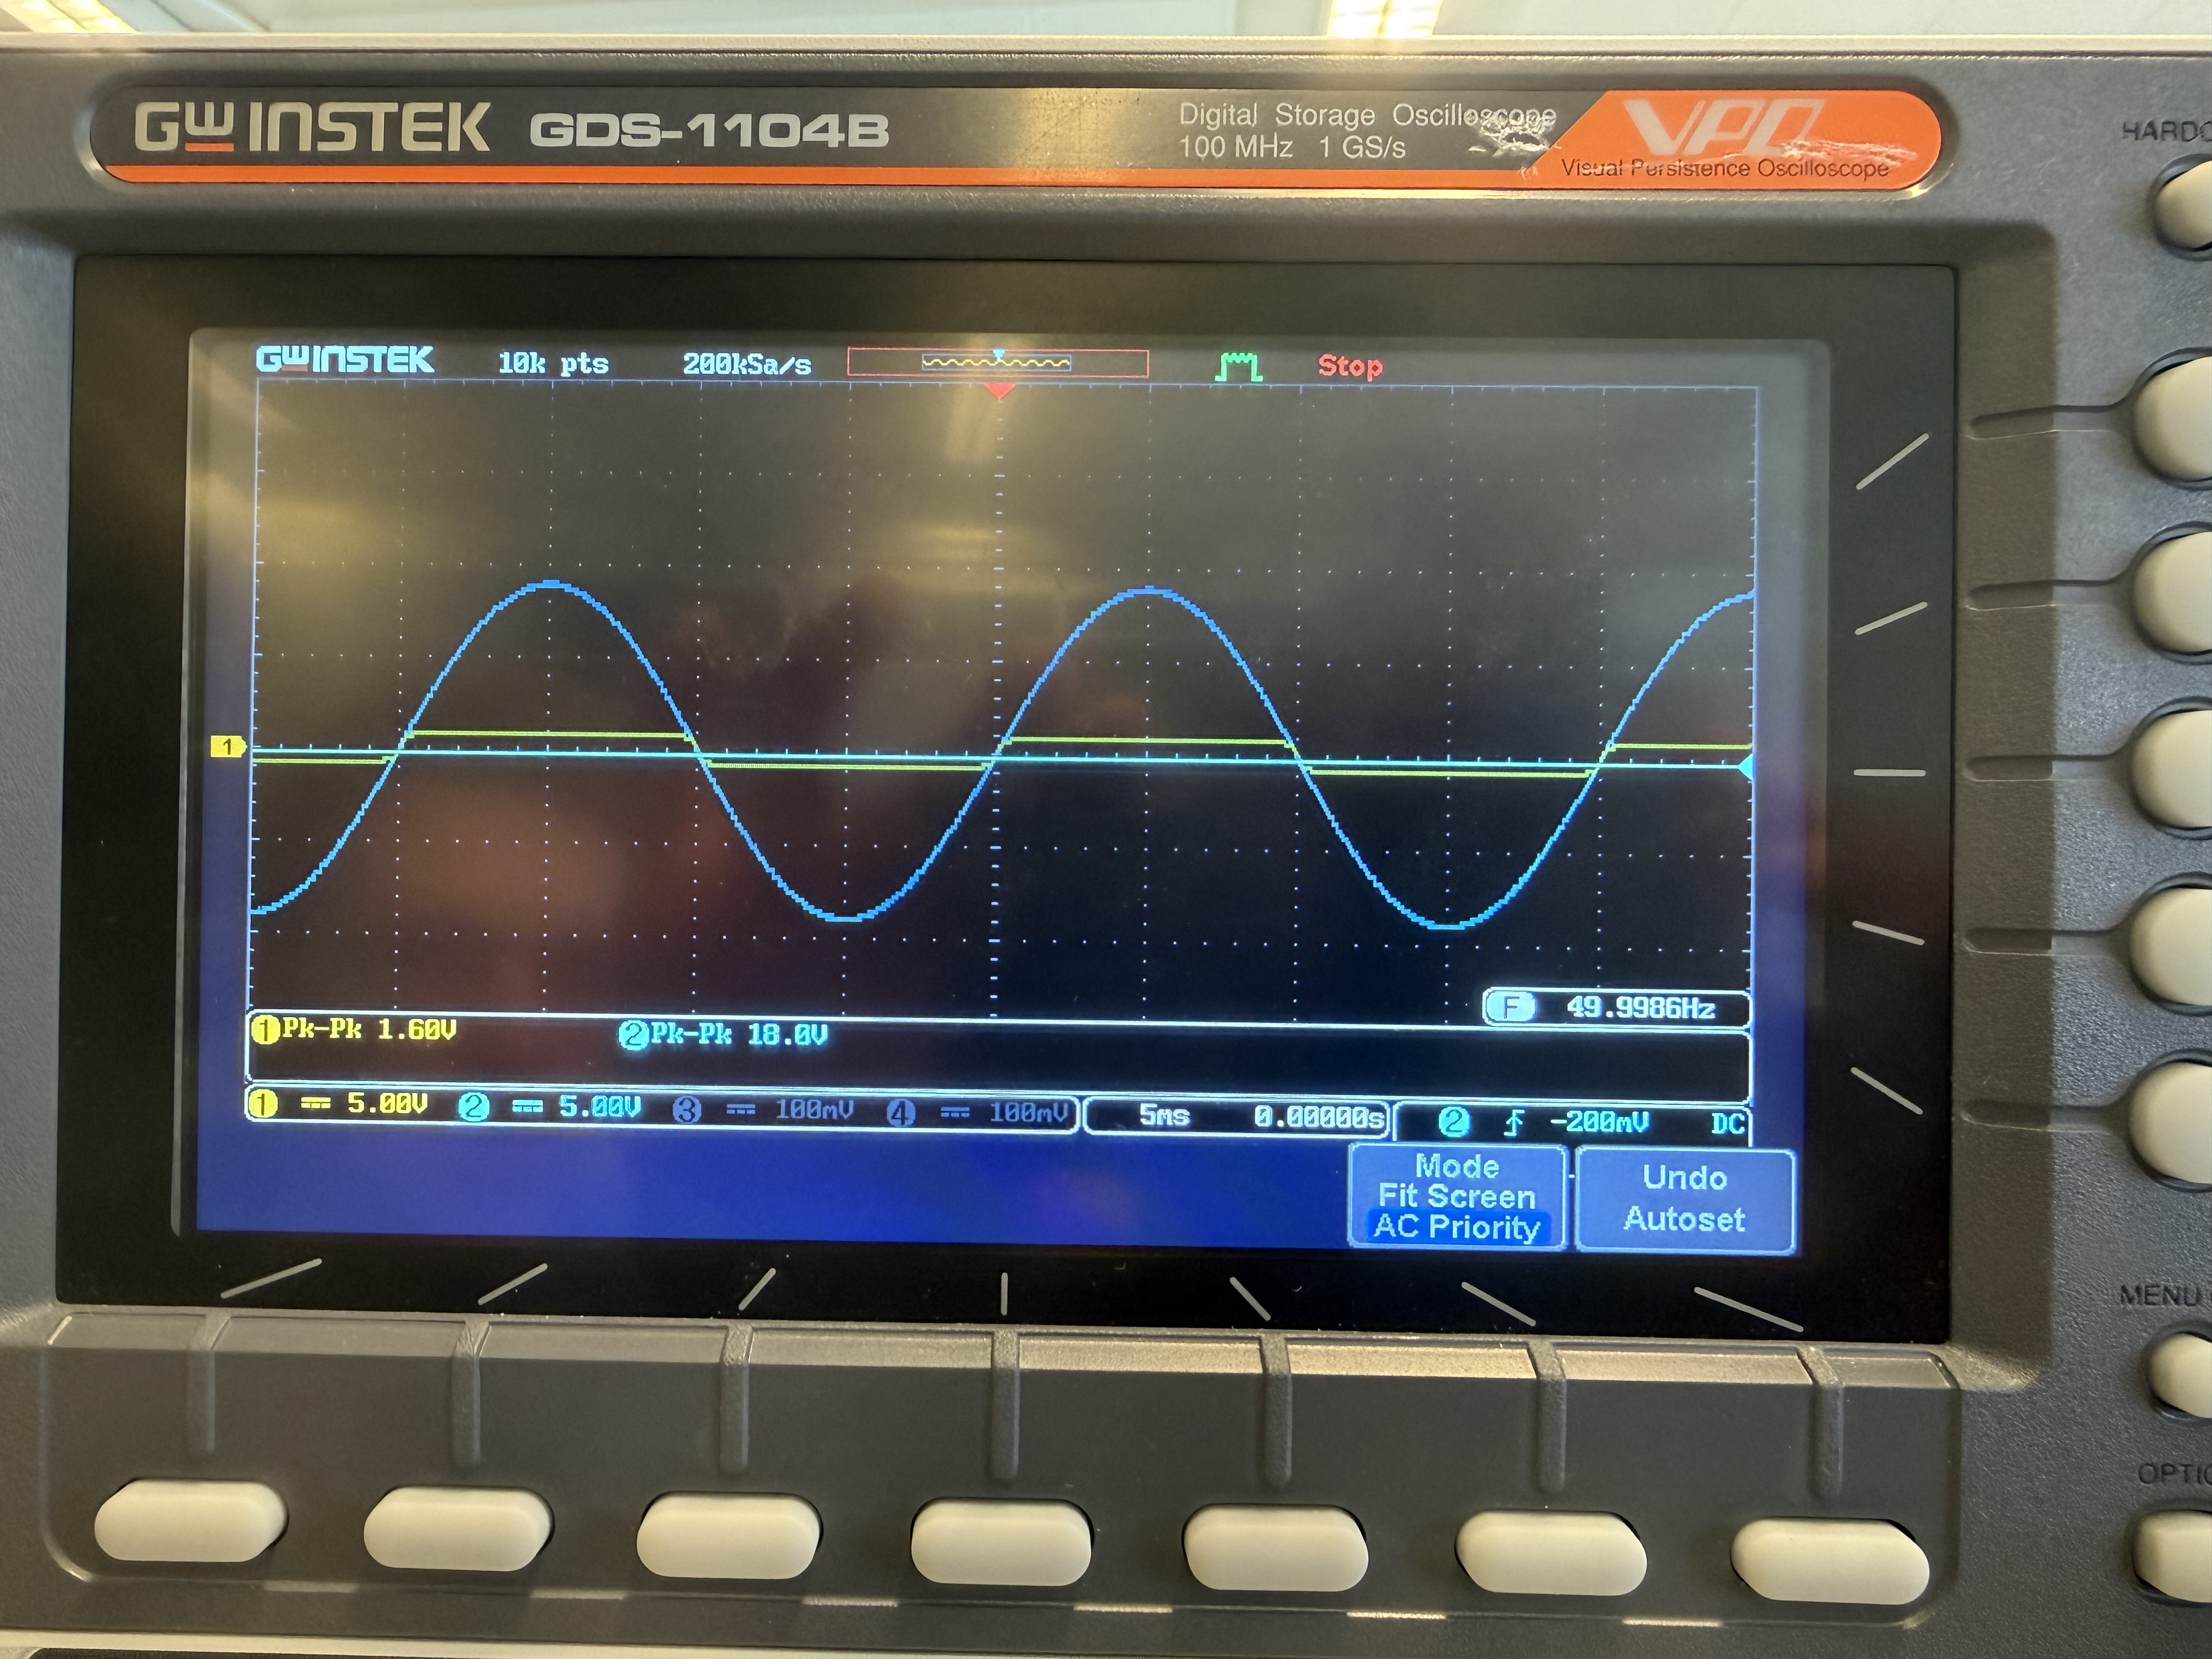
\includegraphics[width=0.7\textwidth]{Media/IMG_0868.jpeg}
            \caption{Måling på utvidet klippekrets}
            \label{fig:utvidet_klippekrets2}
        \end{figure}
        
    \subsection{Måling på klippekrets med zenerdioder}
        I figur \ref{fig:klippekrets_zenerdioder1} skal spenningen $V_{ut}$ over de to zenerdiodene i serie måles. Kretsen divergerer fra kretsen i figur \ref{fig:klippekrets_zenerdioder} ved at $V_{ut}$ faktisk ble målt fra opp til ned som pilen viser i figur \ref{fig:klippekrets_zenerdioder1}, istedenfor ned til opp som det opprinnelig var tenkt. Forventet resultat vil da forventes å være motsatt av den teoretiske kurven fra figur \ref{fig:python_klippekrets_zenerdioder}.
        \begin{figure}[H]
        \centering
        \resizebox{0.7\textwidth}{!}{%
        \begin{circuitikz}
        \tikzstyle{every node}=[font=\fontsize{10.8pt}{14.1pt}\selectfont]
        \draw (6.25,6.75) to[sinusoidal voltage source, sources/symbol/rotate=auto,l={ \fontsize{10.8pt}{14.1pt}\selectfont V1 20Vpp}] (6.25,11.75);
        \draw (13.75,9.25) to[empty Zener diode] (13.75,6.75);
        \draw (13.75,9.25) to[empty Zener diode,l={ \fontsize{10.8pt}{14.1pt}\selectfont D4 C4V7}] (13.75,11.75);
        \draw (6.25,6.75) to[short] (13.75,6.75);
        \node [font=\fontsize{10.8pt}{14.1pt}\selectfont, inner xsep=0.080cm, inner ysep=0.085cm, rounded corners=0.020cm] at (12.625,8) {D5 C6V8};
        \draw [-{Stealth[scale=1.5]}, ] (15,11.75) -- (15,7.25);
        \node [font=\fontsize{10.8pt}{14.1pt}\selectfont, inner xsep=0.080cm, inner ysep=0.085cm, rounded corners=0.020cm] at (15.5,9.5) {$V_{ut}$};
        \draw (6.25,11.75) to[R,l={ \fontsize{10.8pt}{14.1pt}\selectfont R1 180$\Omega$}] (13.75,11.75);
        \end{circuitikz}
        }%
        \caption{Klippekrets med zenerdioder}
        \label{fig:klippekrets_zenerdioder1}
        \end{figure}

        I figur \ref{fig:klippekrets_zenerdioder2} ser man spenningskurvene for inngangssignalet $V1$ og $V_{ut}$. Som forventet er den gule kurven, altså $V_{ut}$, motsatt fra kurven i figur \ref{fig:python_klippekrets_zenerdioder}.
        I positiv halvperiode klippes spenningen til omtrent i underkant av $6V$ istedenfor $-5.4V$, mens i negativ halvperiode klippes spenningen til omtrent $-7.5V$ istedenfor $7.5V$.
        Generelt sett så stemmer de teoretiske beregningene i henhold til de praktiske målingene, men på grunn av måten $V_{ut}$ måles på så fremstår målingene som motsatt.
        \begin{figure}[H]
            \centering
            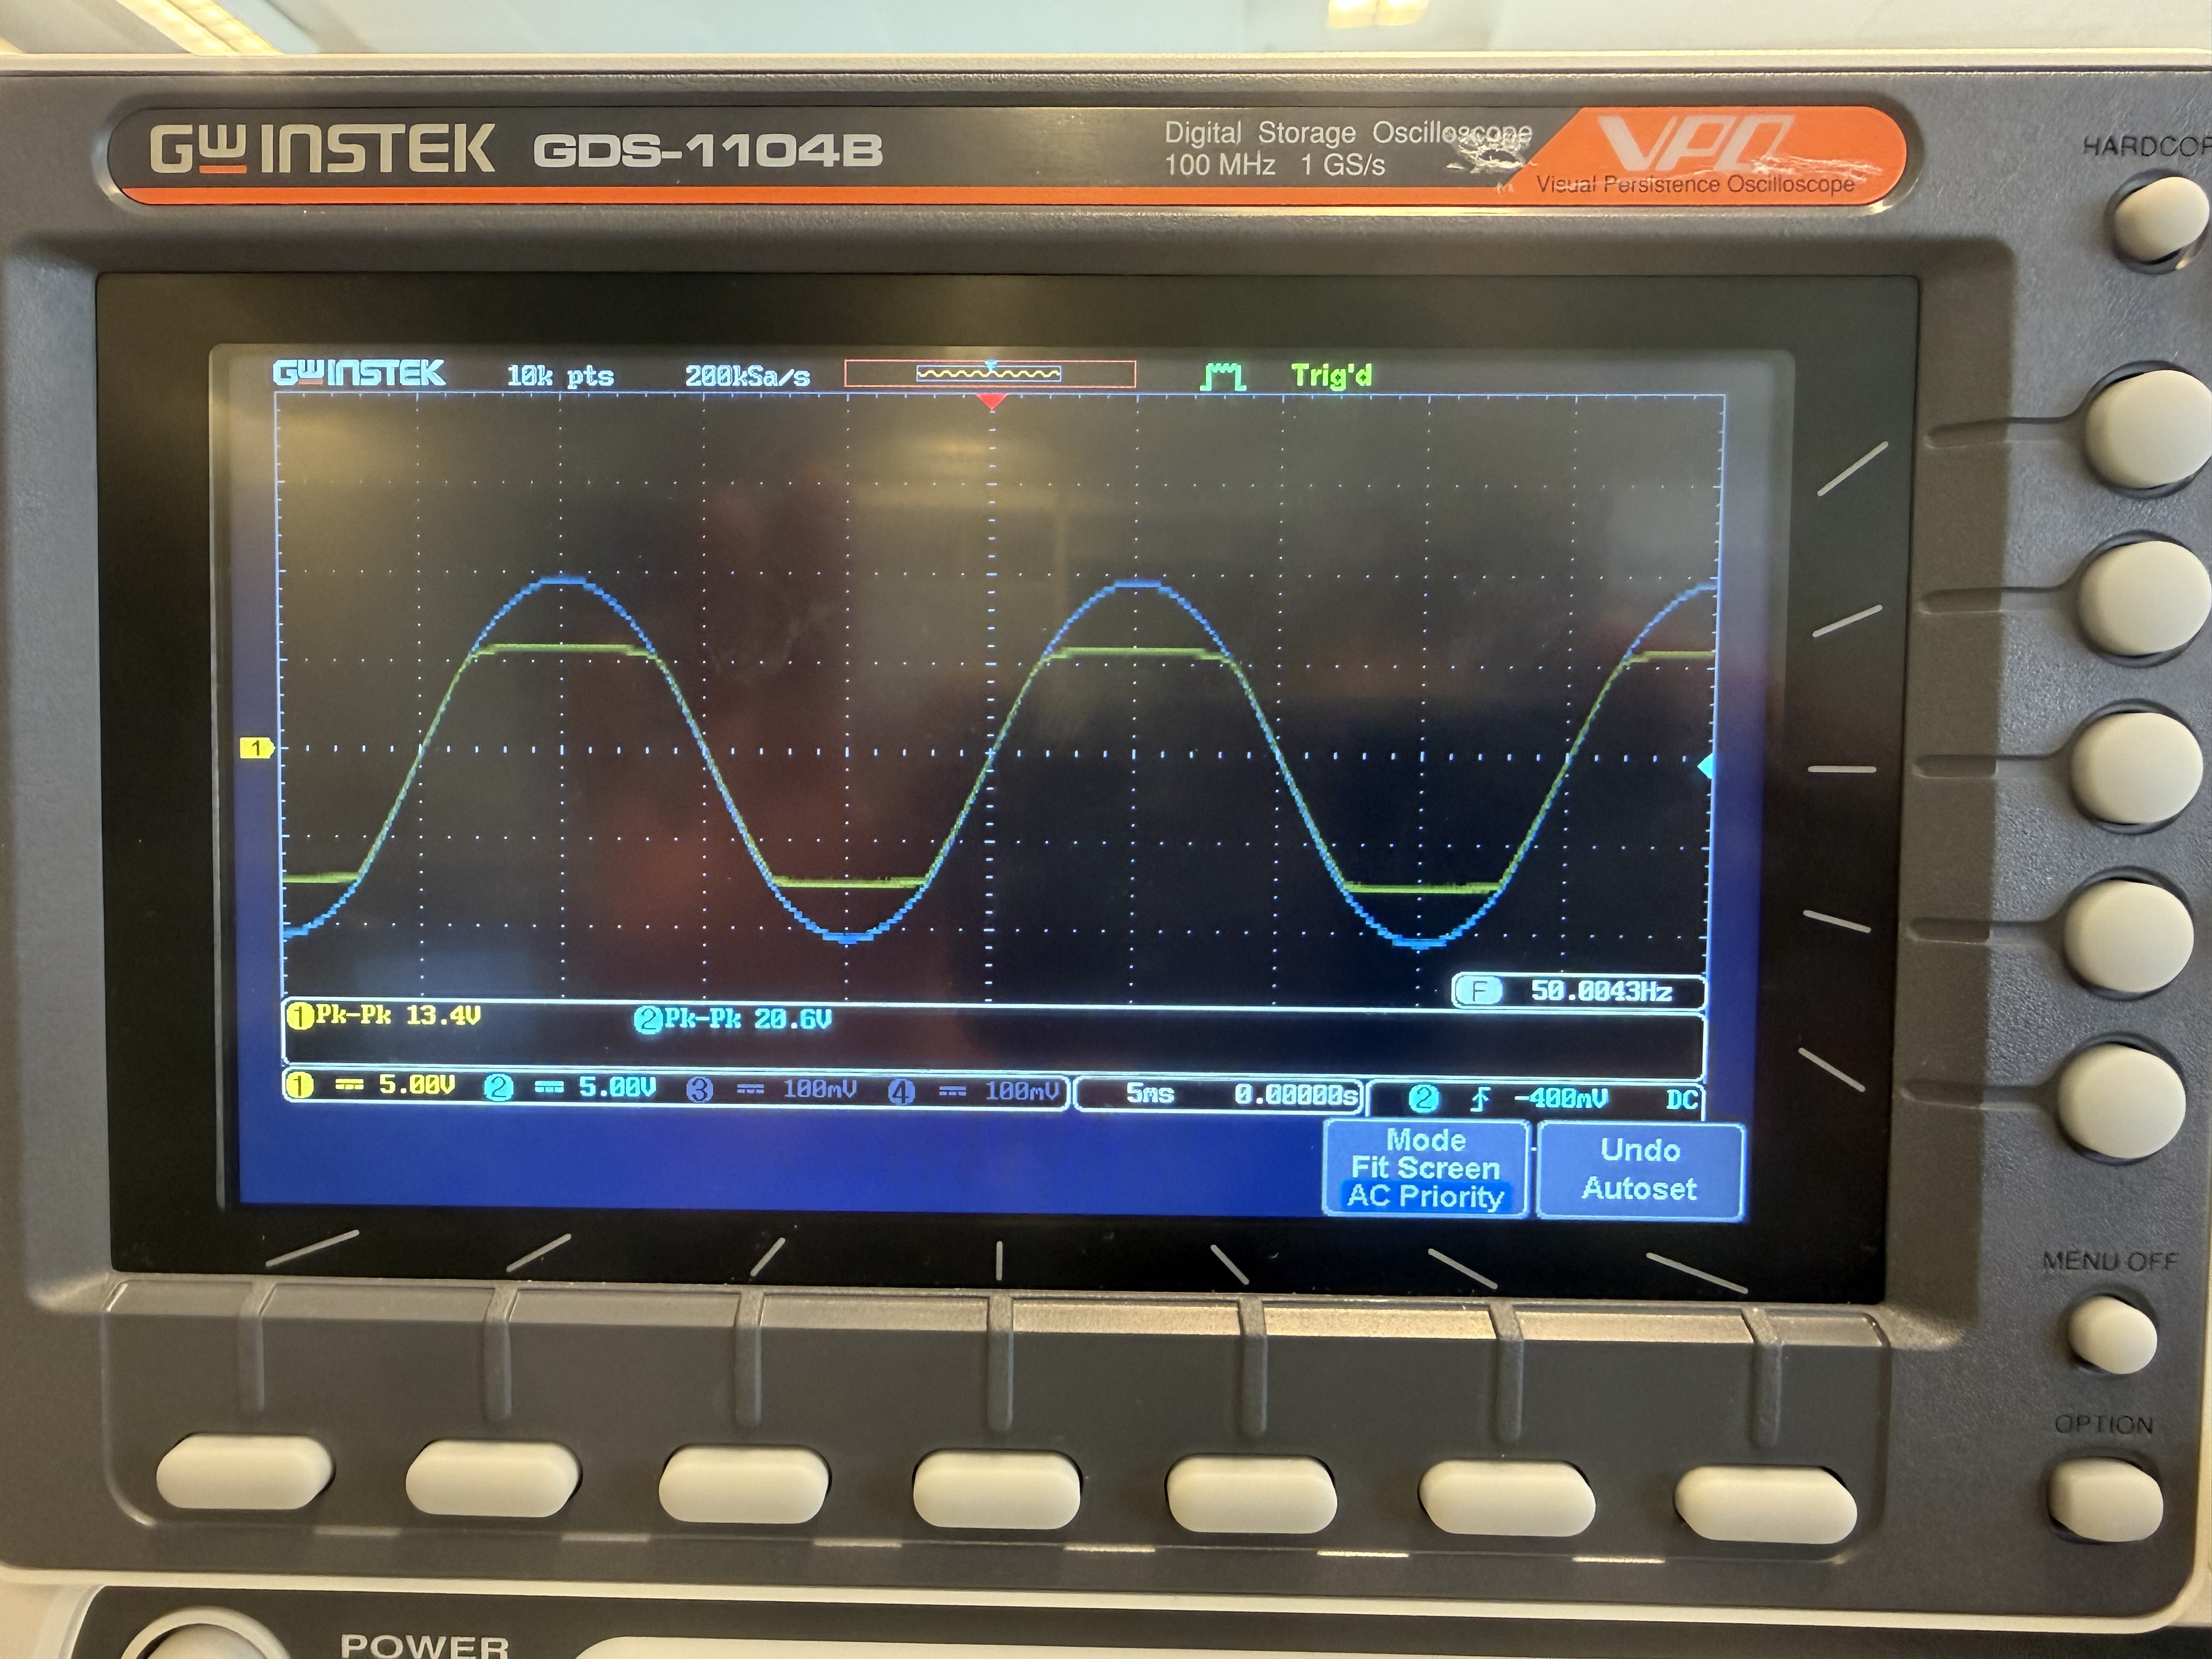
\includegraphics[width=0.7\textwidth]{Media/IMG_0869.jpeg}
            \caption{Måling på klippekrets med zenerdioder}
            \label{fig:klippekrets_zenerdioder2}
        \end{figure}
        
    \subsection{Målinger på kretser for enveis likeretting}
        \subsubsection{Enveis likeretting}
            \begin{figure}[H]
                \centering
                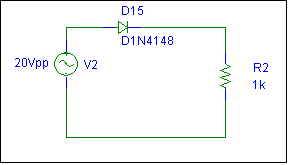
\includegraphics[width=0.7\textwidth]{Media/enveis_likeretting.png}
                \caption{Enveis likeretter}
                \label{fig:enveis_likeretter1}
            \end{figure}

            \begin{figure}[H]
                \centering
                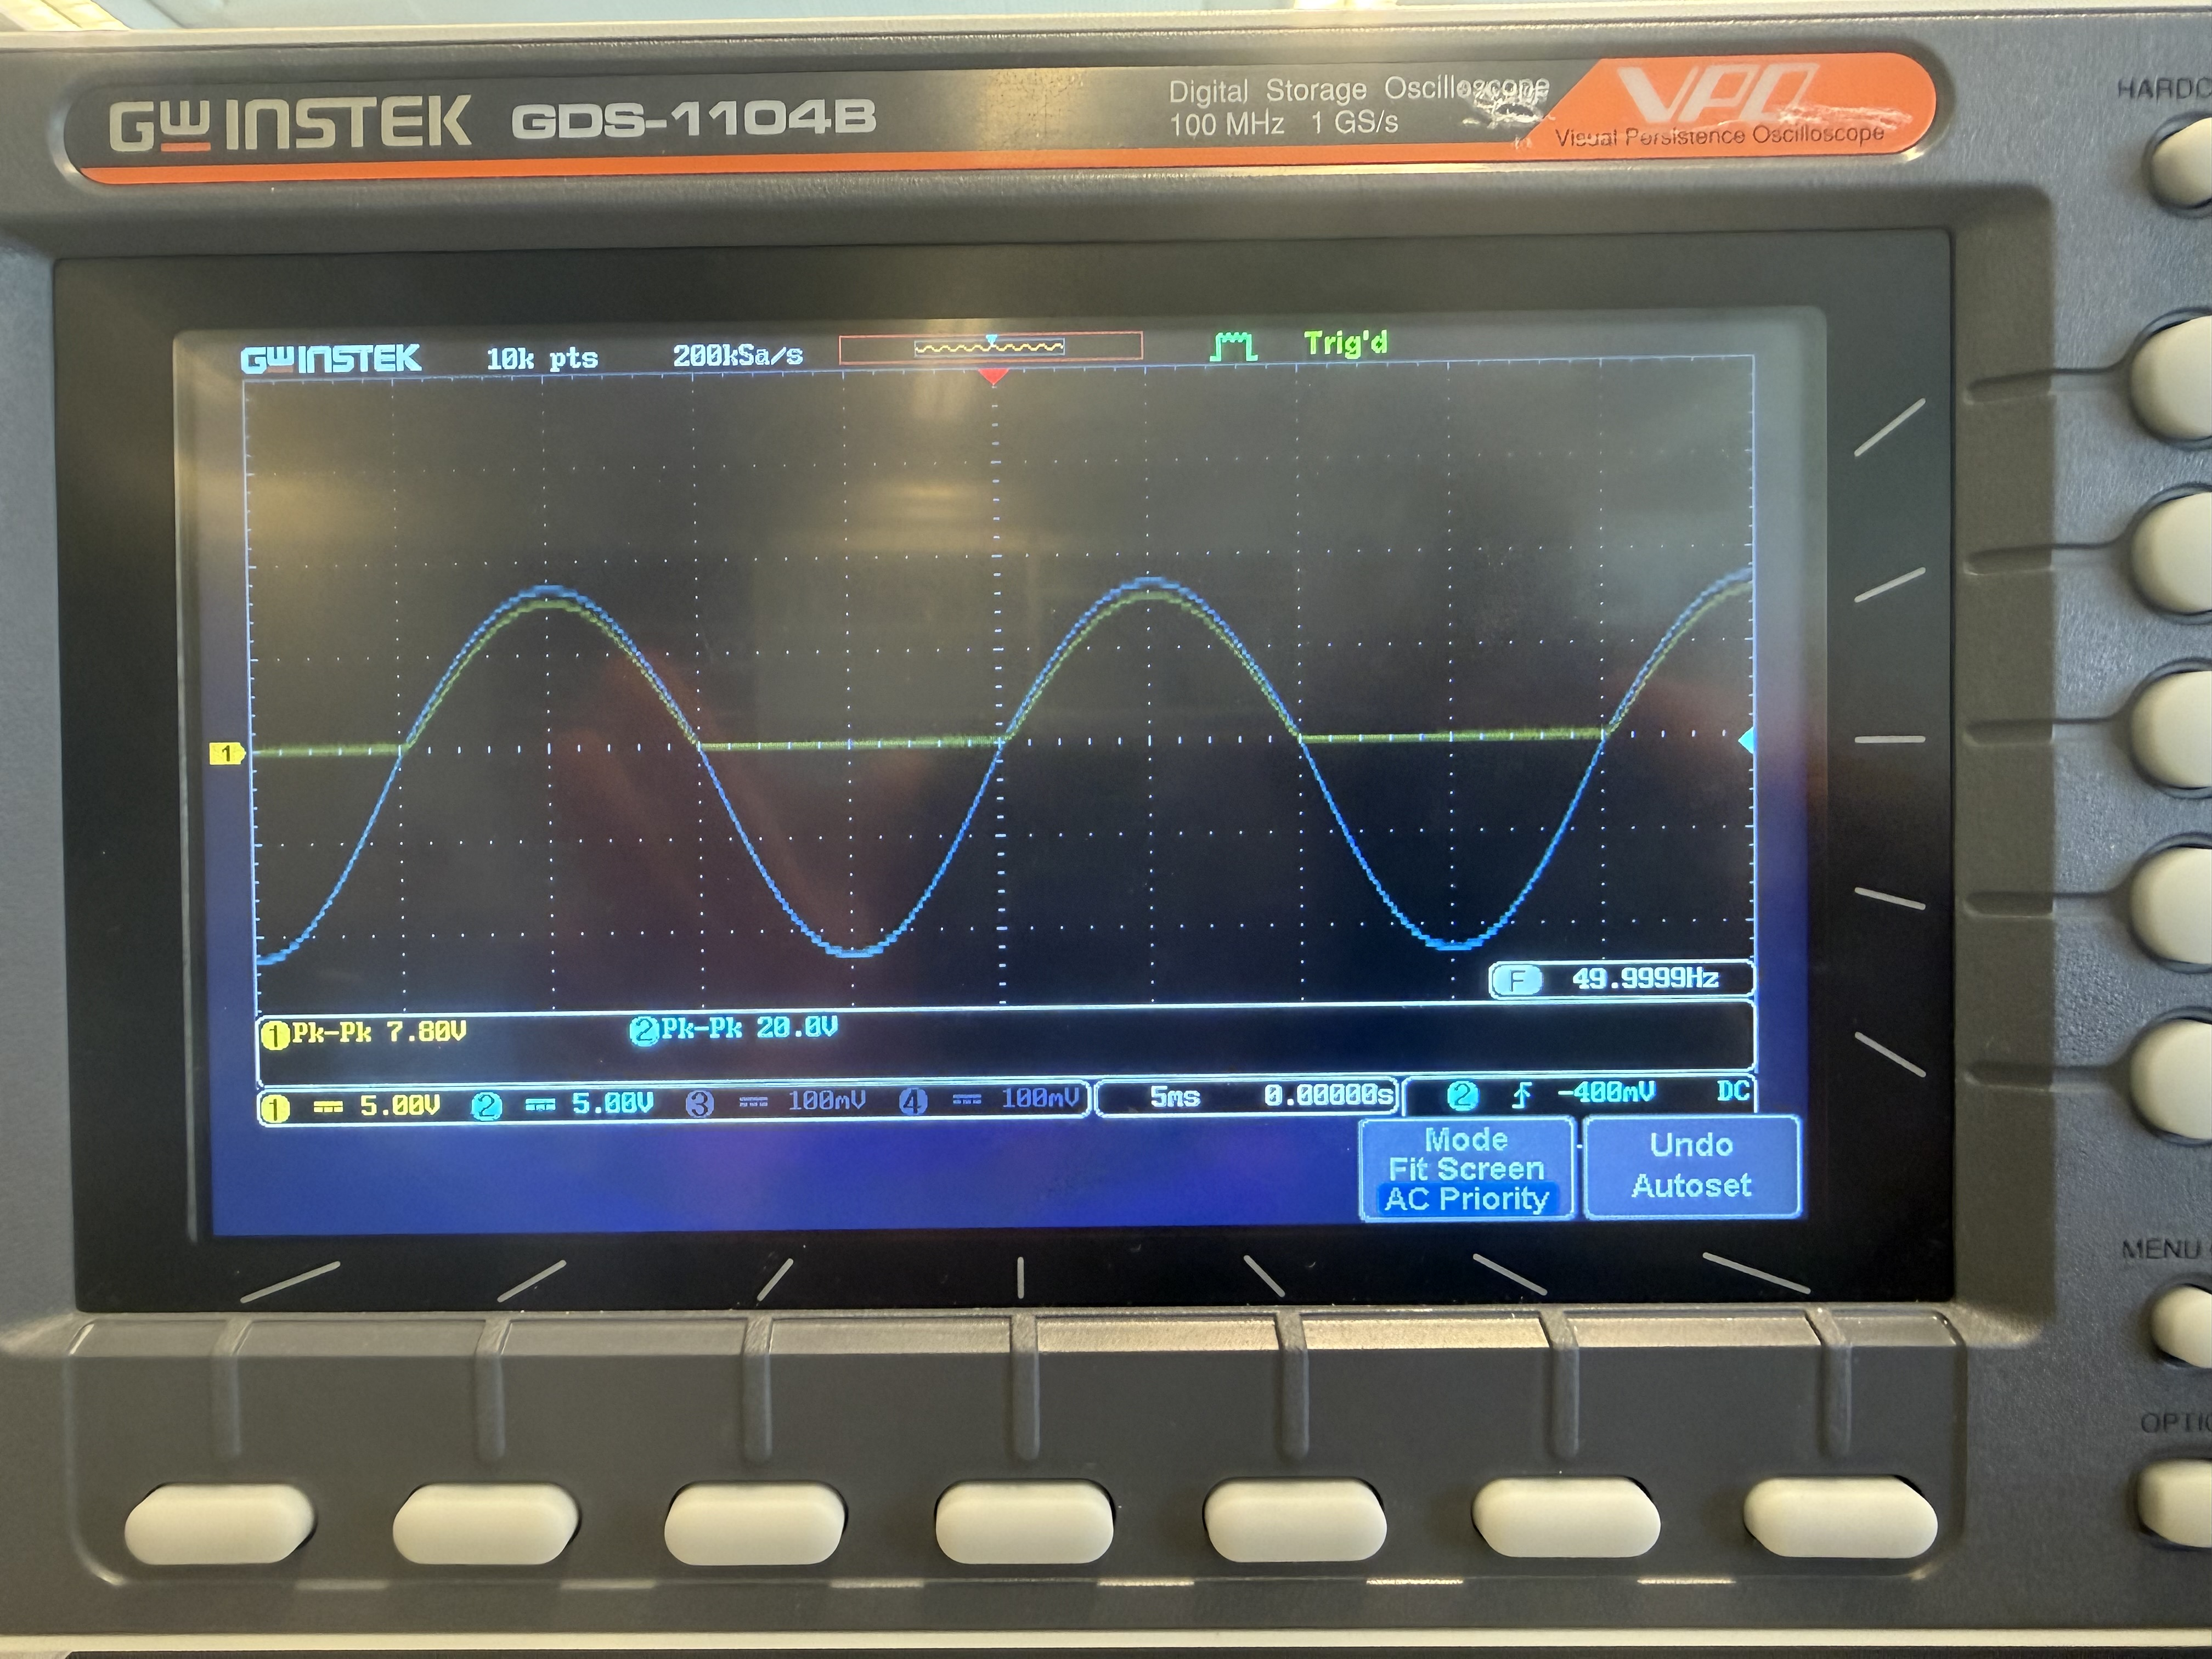
\includegraphics[width=0.7\textwidth]{Media/IMG_0870.jpeg}
                \caption{Måling på spenningen over $R2$}
                \label{fig:enveis_likeretter2}
            \end{figure}

            \subsubsection{Enveis likeretting: dioden snudd}
                \begin{figure}[H]
                    \centering
                    \resizebox{0.7\textwidth}{!}{%
                    \begin{circuitikz}
                    \tikzstyle{every node}=[font=\fontsize{10.8pt}{14.1pt}\selectfont]
                    \draw (12.5,14) to[D,l={ \fontsize{10.8pt}{14.1pt}\selectfont D15}] (10,14);
                    \draw (12.5,14) to[short] (13.75,14);
                    \draw (13.75,14) to[R,l={ \fontsize{10.8pt}{14.1pt}\selectfont R2}] (13.75,10.25);
                    \draw (10,10.25) to[short] (13.75,10.25);
                    \draw (10,14) to[short] (8.75,14);
                    \draw (8.75,14) to[sinusoidal voltage source, sources/symbol/rotate=auto,l={ \fontsize{10.8pt}{14.1pt}\selectfont \textbf{V2}}] (8.75,10.25);
                    \draw (8.75,10.25) to[short] (10.125,10.25);
                    \node [font=\fontsize{10.8pt}{14.1pt}\selectfont, inner xsep=0.080cm, inner ysep=0.085cm, rounded corners=0.020cm] at (7.625,12.125) {20Vpp};
                    \node [font=\fontsize{10.8pt}{14.1pt}\selectfont, inner xsep=0.080cm, inner ysep=0.085cm, rounded corners=0.020cm] at (11.375,14.625) {D1N4148};
                    \node [font=\fontsize{10.8pt}{14.1pt}\selectfont, inner xsep=0.080cm, inner ysep=0.085cm, rounded corners=0.020cm] at (13,12.125) {1k$\Omega$};
                    \end{circuitikz}
                    }%
                    \caption{Dioden byttet vei: enkel likeretter}
                    \label{fig:flip_diode_enkel_likeretter1}
                \end{figure}

                \begin{figure}[H]
                    \centering
                    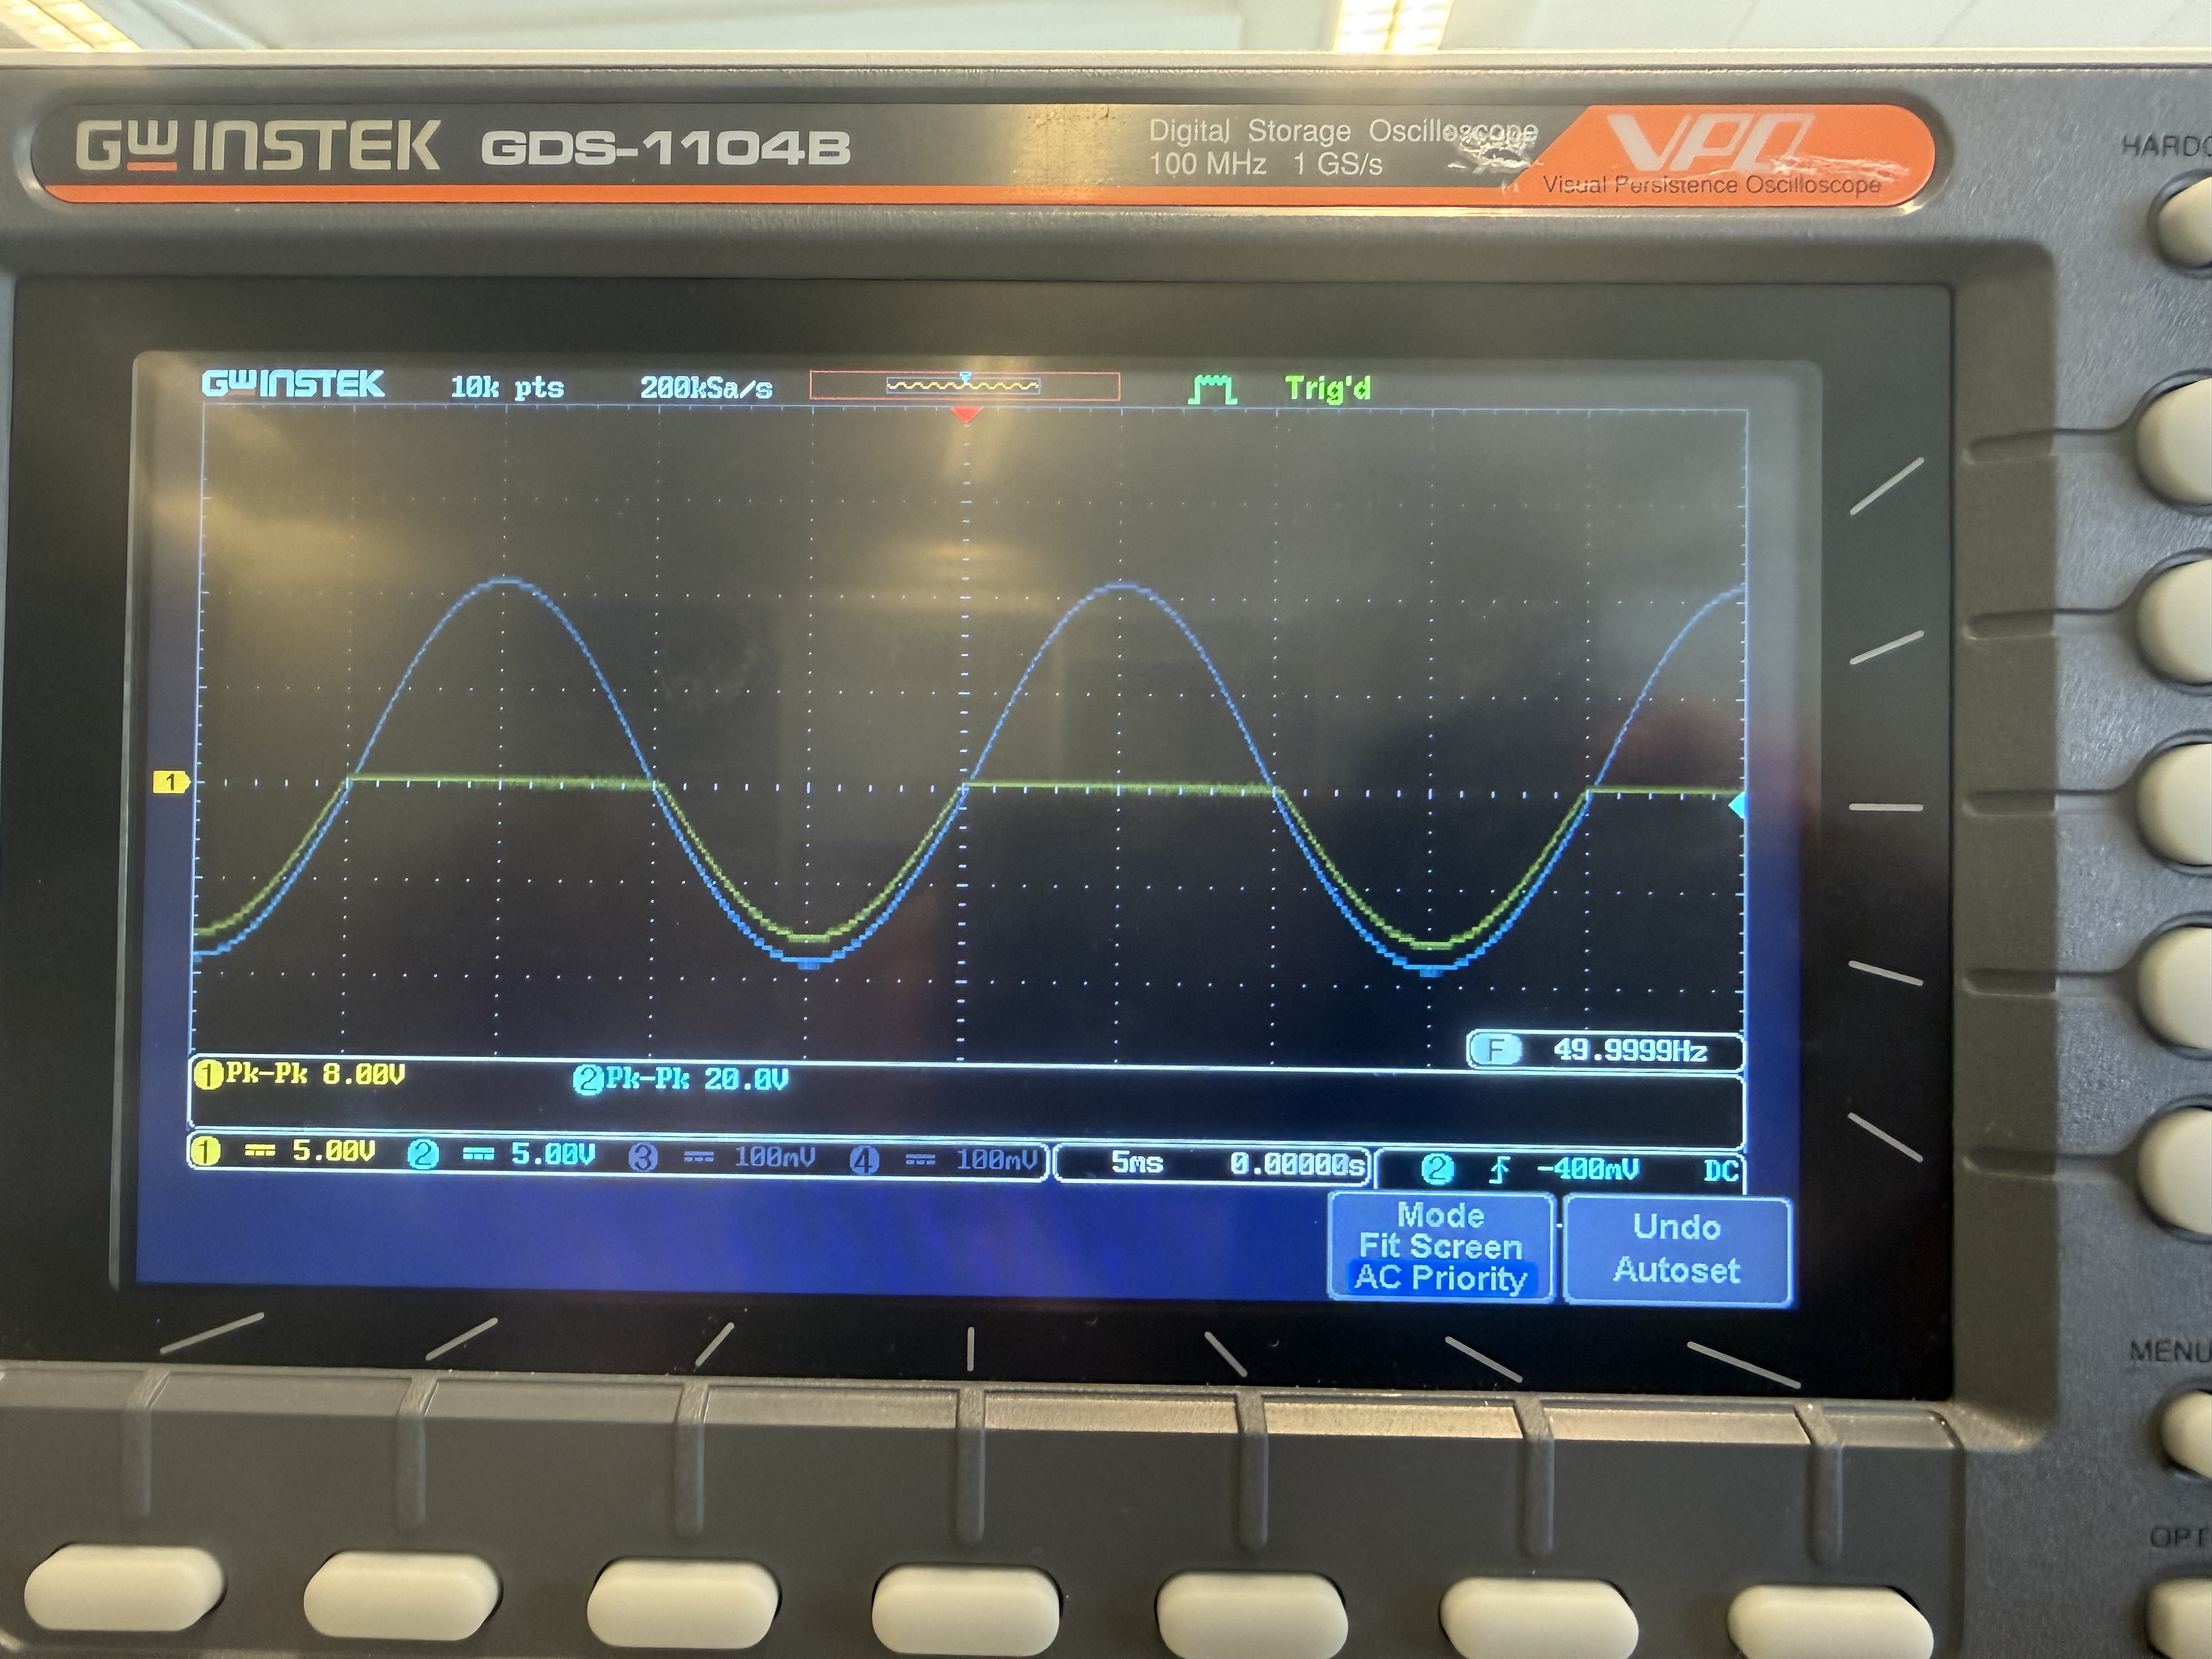
\includegraphics[width=0.7\textwidth]{Media/IMG_0871.jpeg}
                    \caption{Måling på spenningen over $R2$}
                    \label{fig:flip_diode_enkel_likeretter2}
                \end{figure}
    \subsection{Målinger på krets for toveis likeretting}
        230V transformator brukt
        \begin{figure}[H]
            \centering
            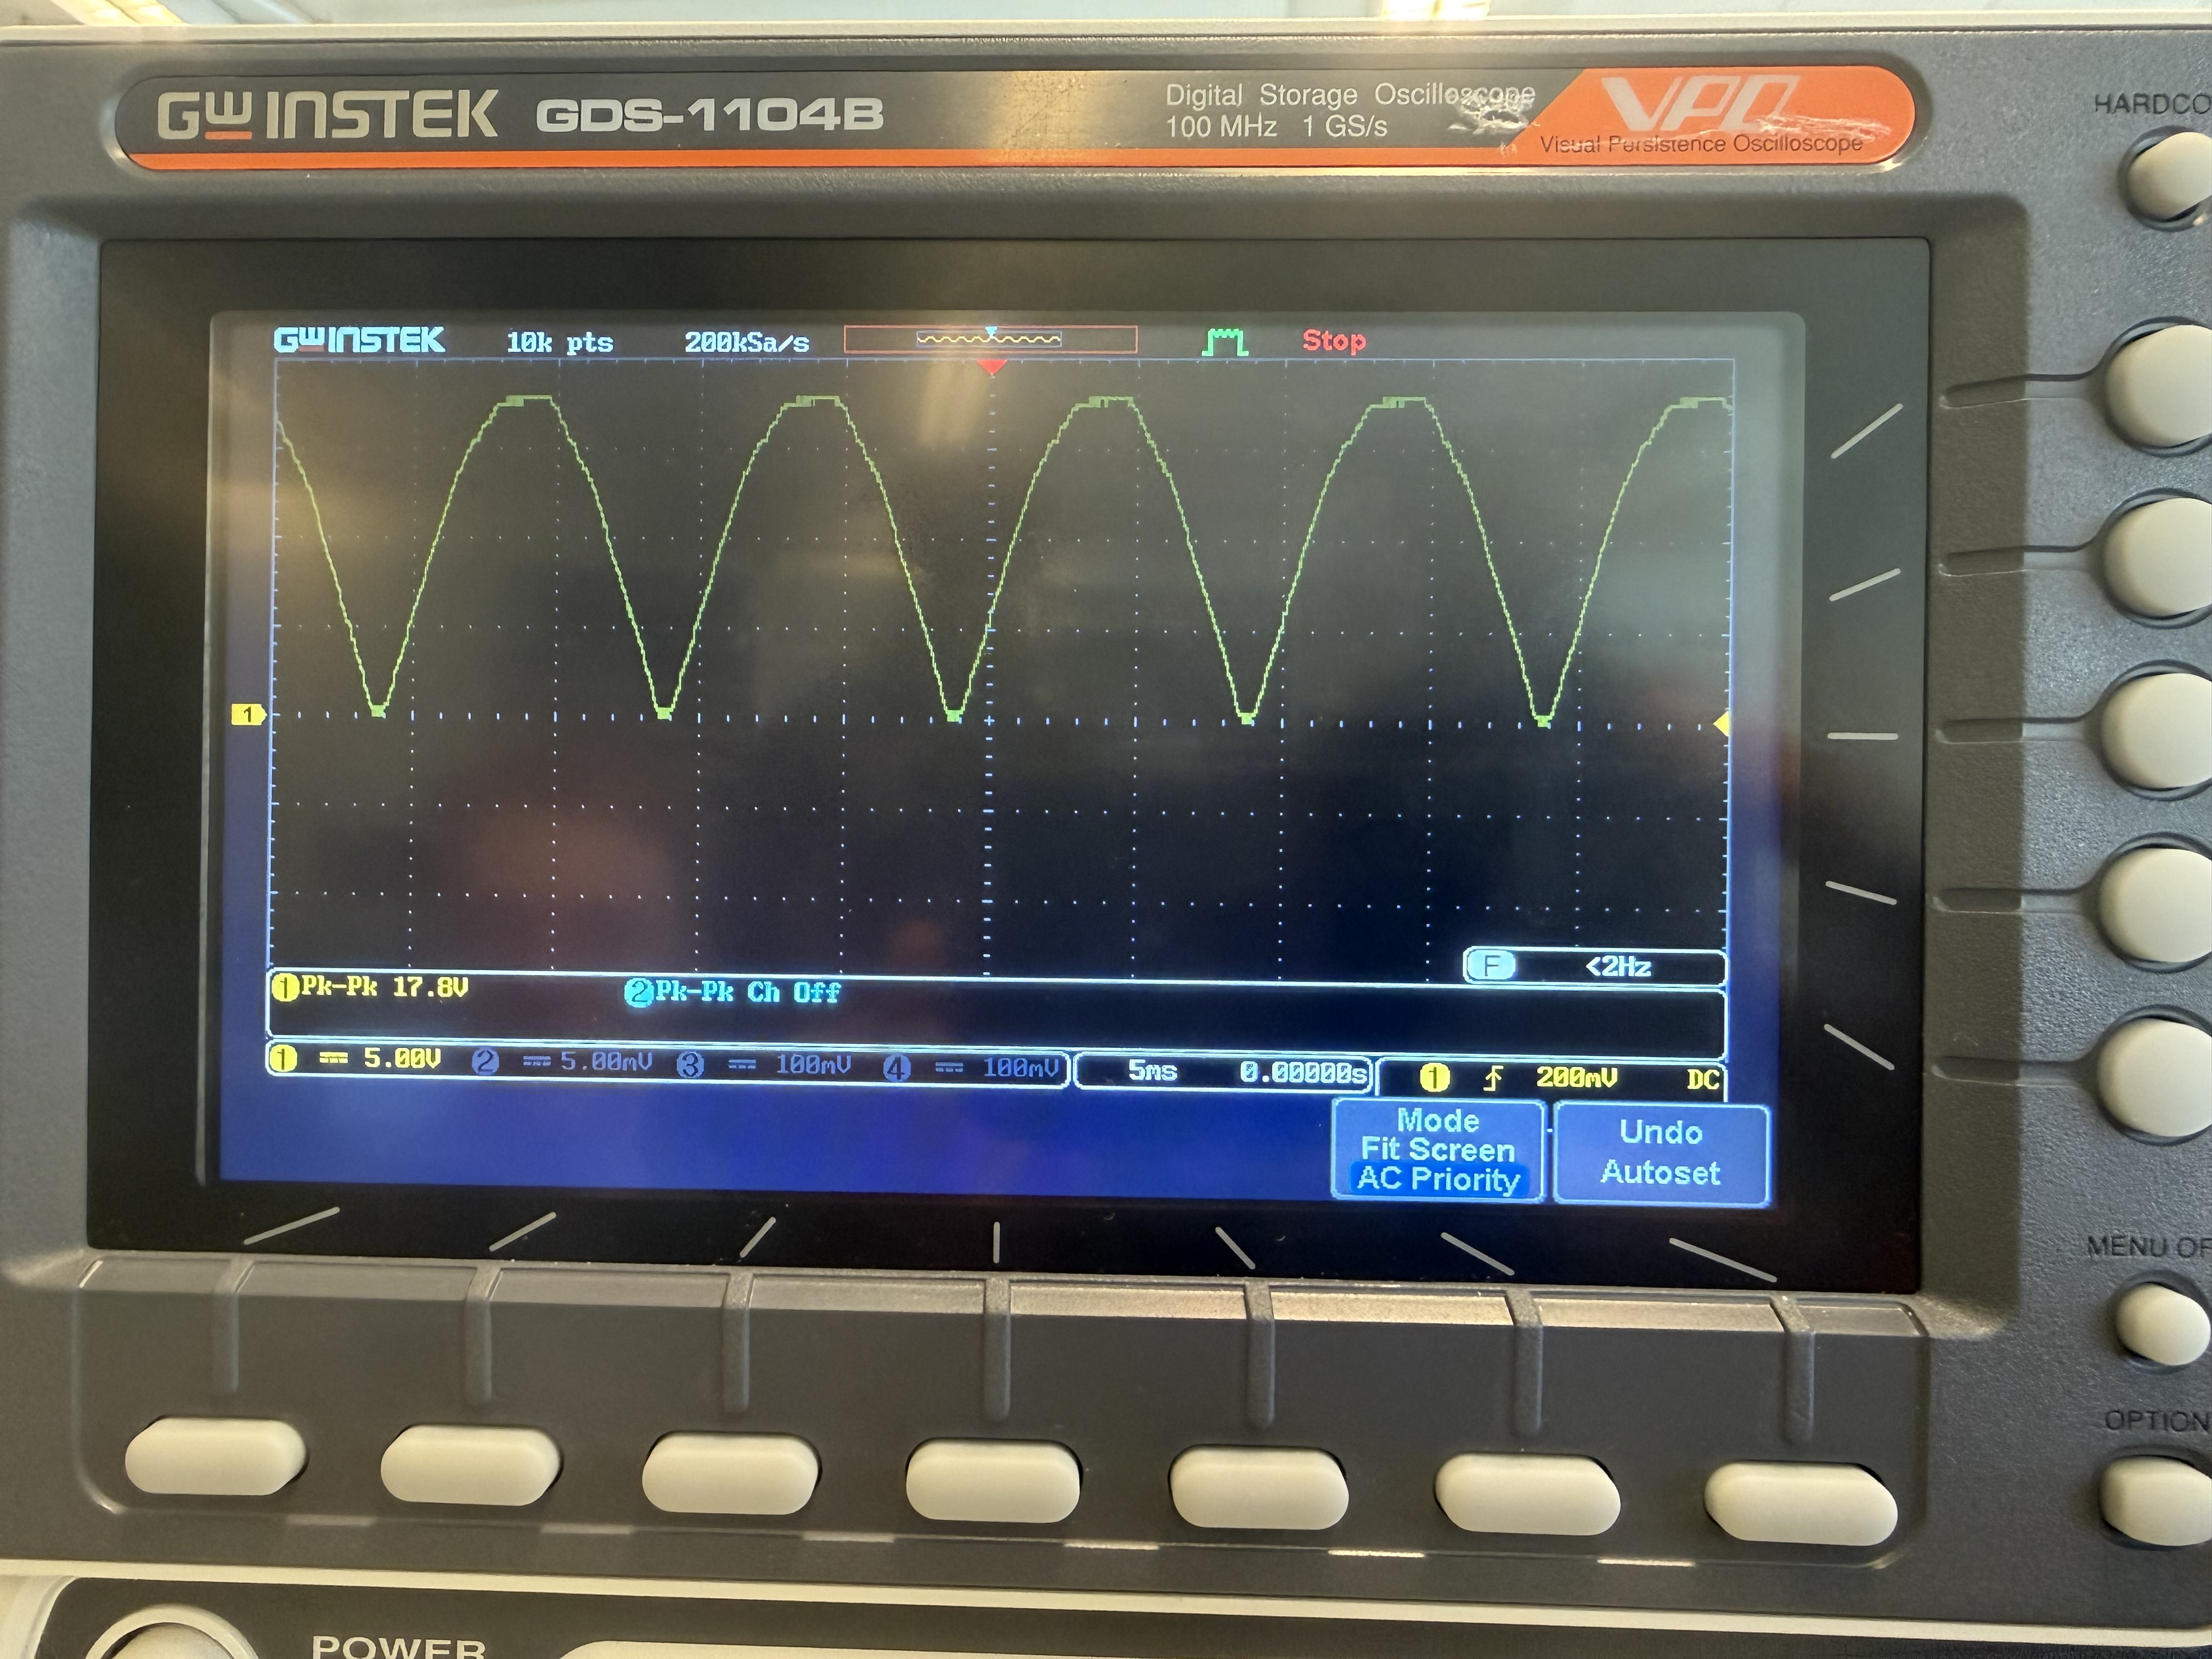
\includegraphics[width=0.7\textwidth]{Media/IMG_0873.jpeg}
            \caption{Måling på spenningen over $R4$}
            \label{fig:toveis_likeretting_transformator}
        \end{figure}
        
    \subsection{Målinger på krets for toveis likeretter med RC-ledd}
        \subsubsection{RC-ledd: $C2 = 100\mu F$}
            \begin{figure}[H]
                \centering
                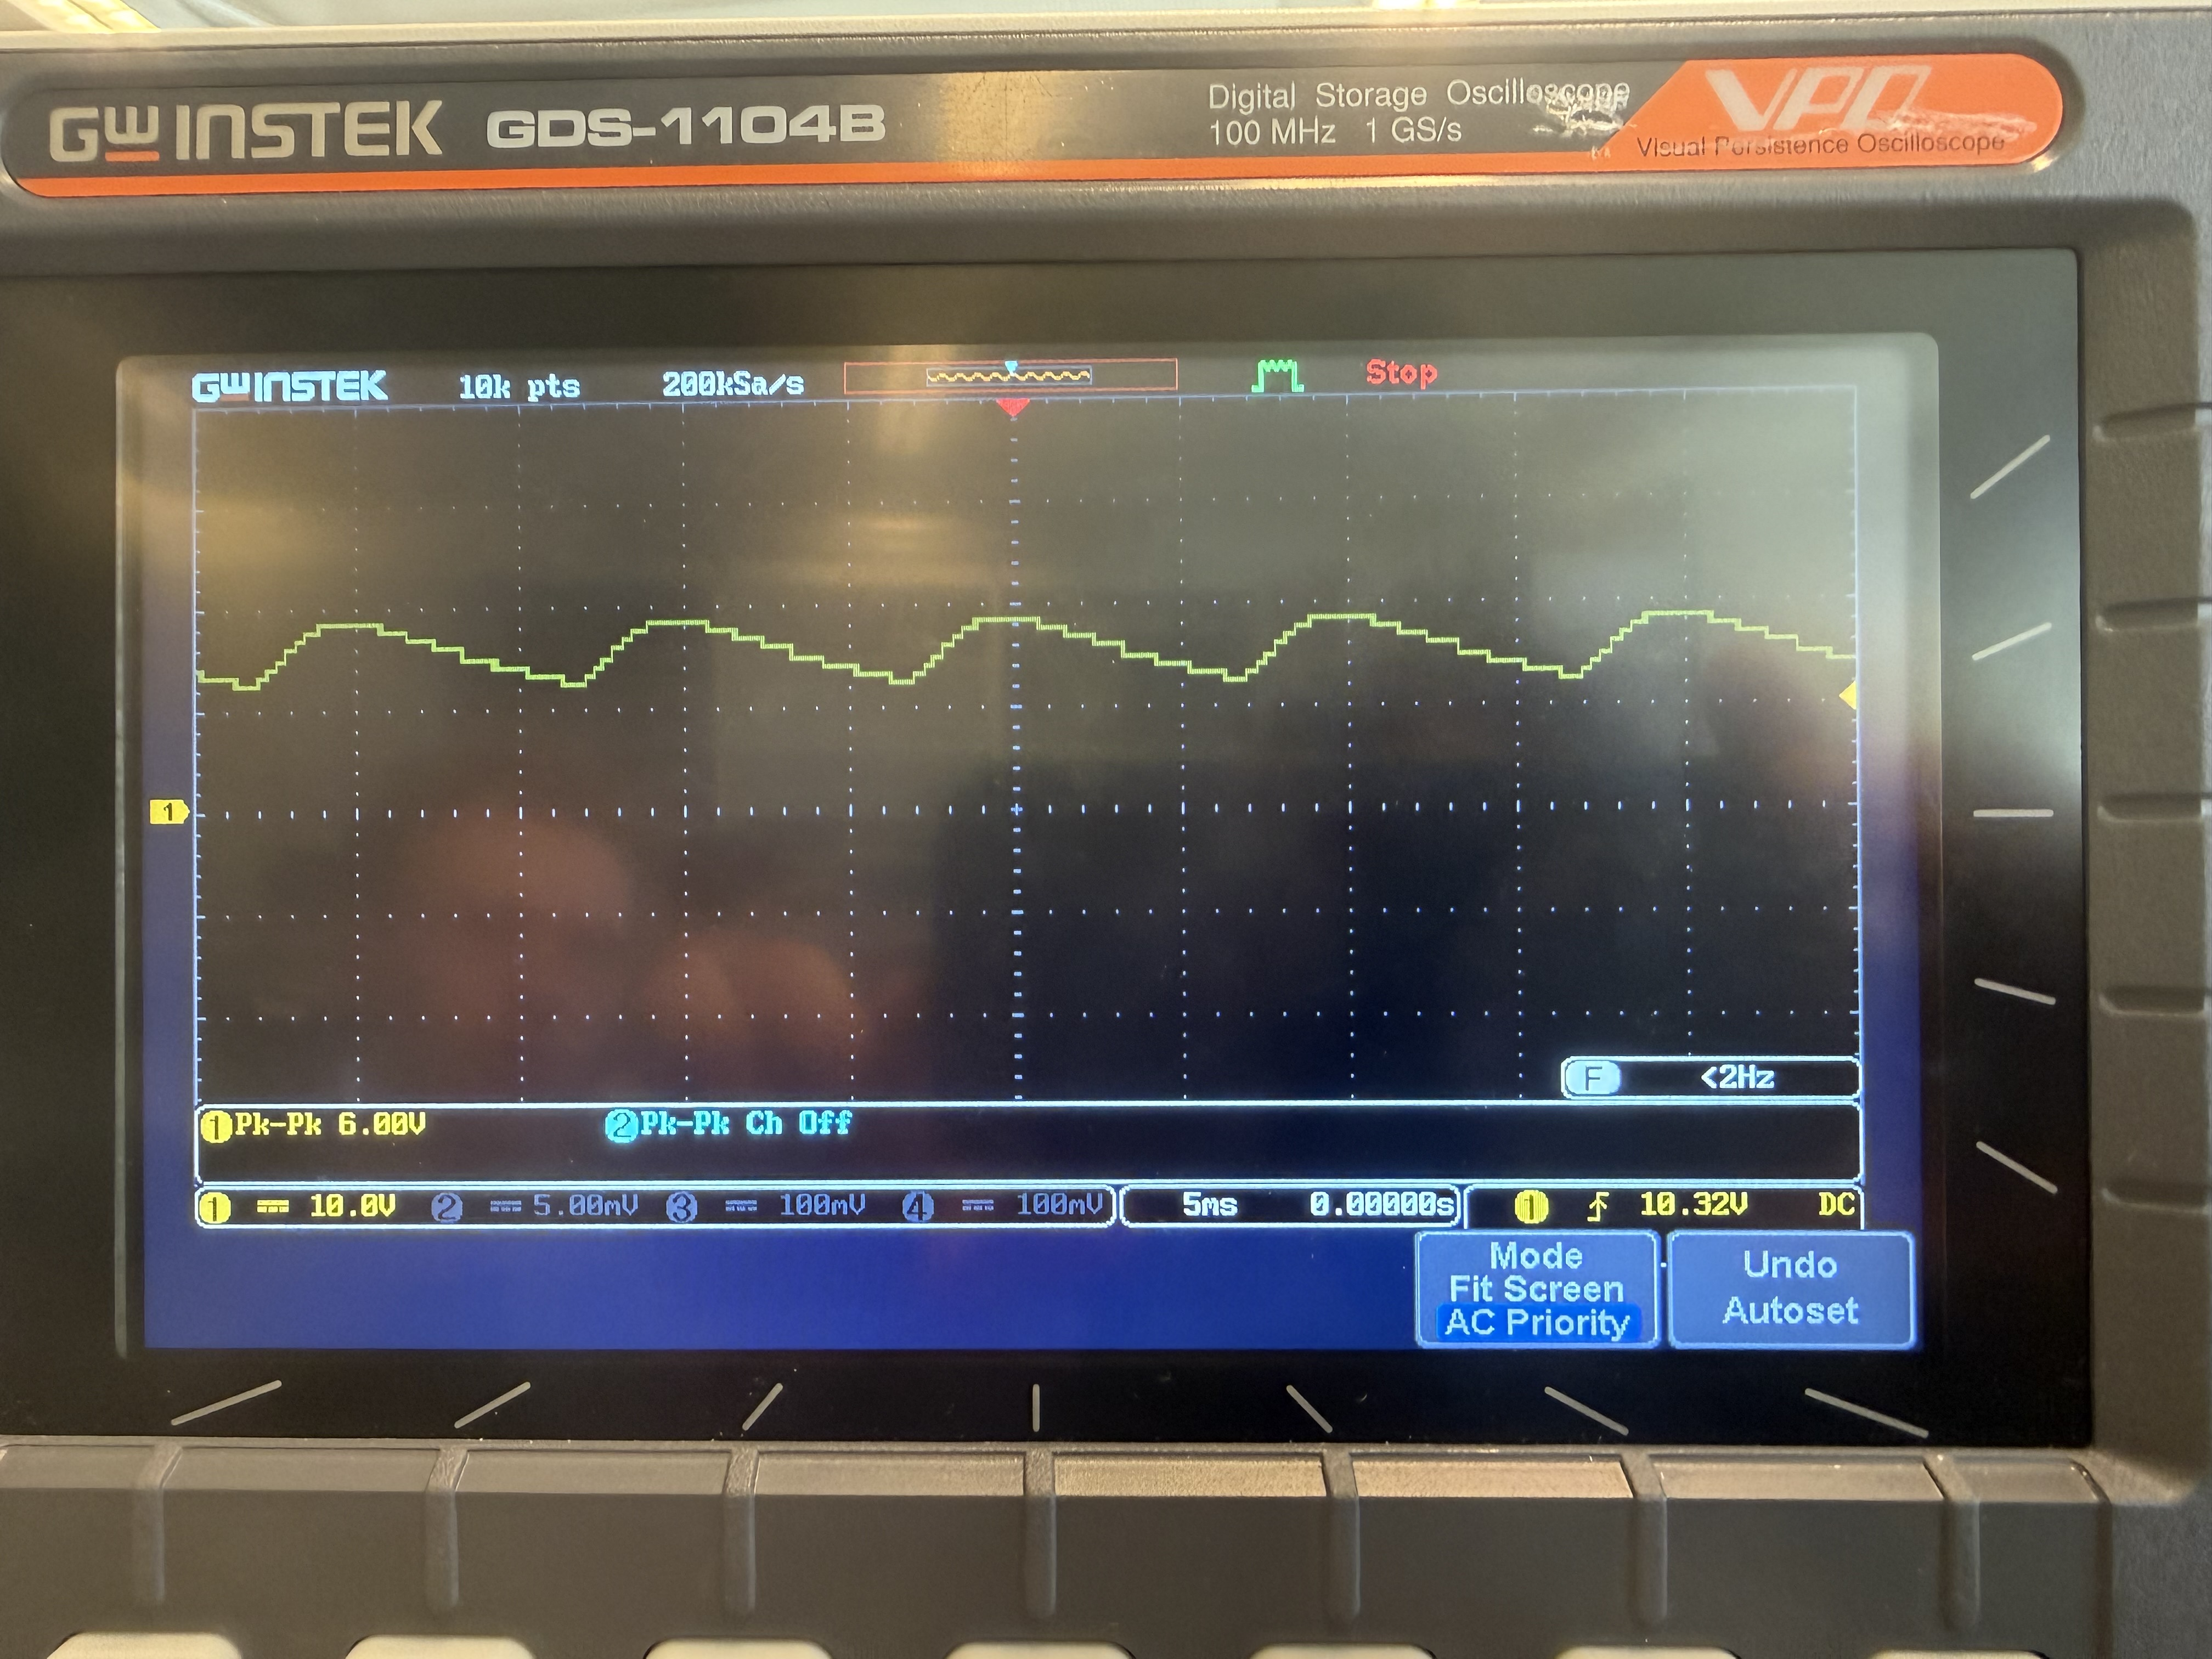
\includegraphics[width=0.7\textwidth]{Media/IMG_0874.jpeg}
                \caption{DC-mode: måling på spenningen over RC-leddet med $100\mu F$}
                \label{fig:toveis_likeretting_transformator_RC1}
            \end{figure}
            Ser hele signalet med DC-mode

            \begin{figure}[H]
                \centering
                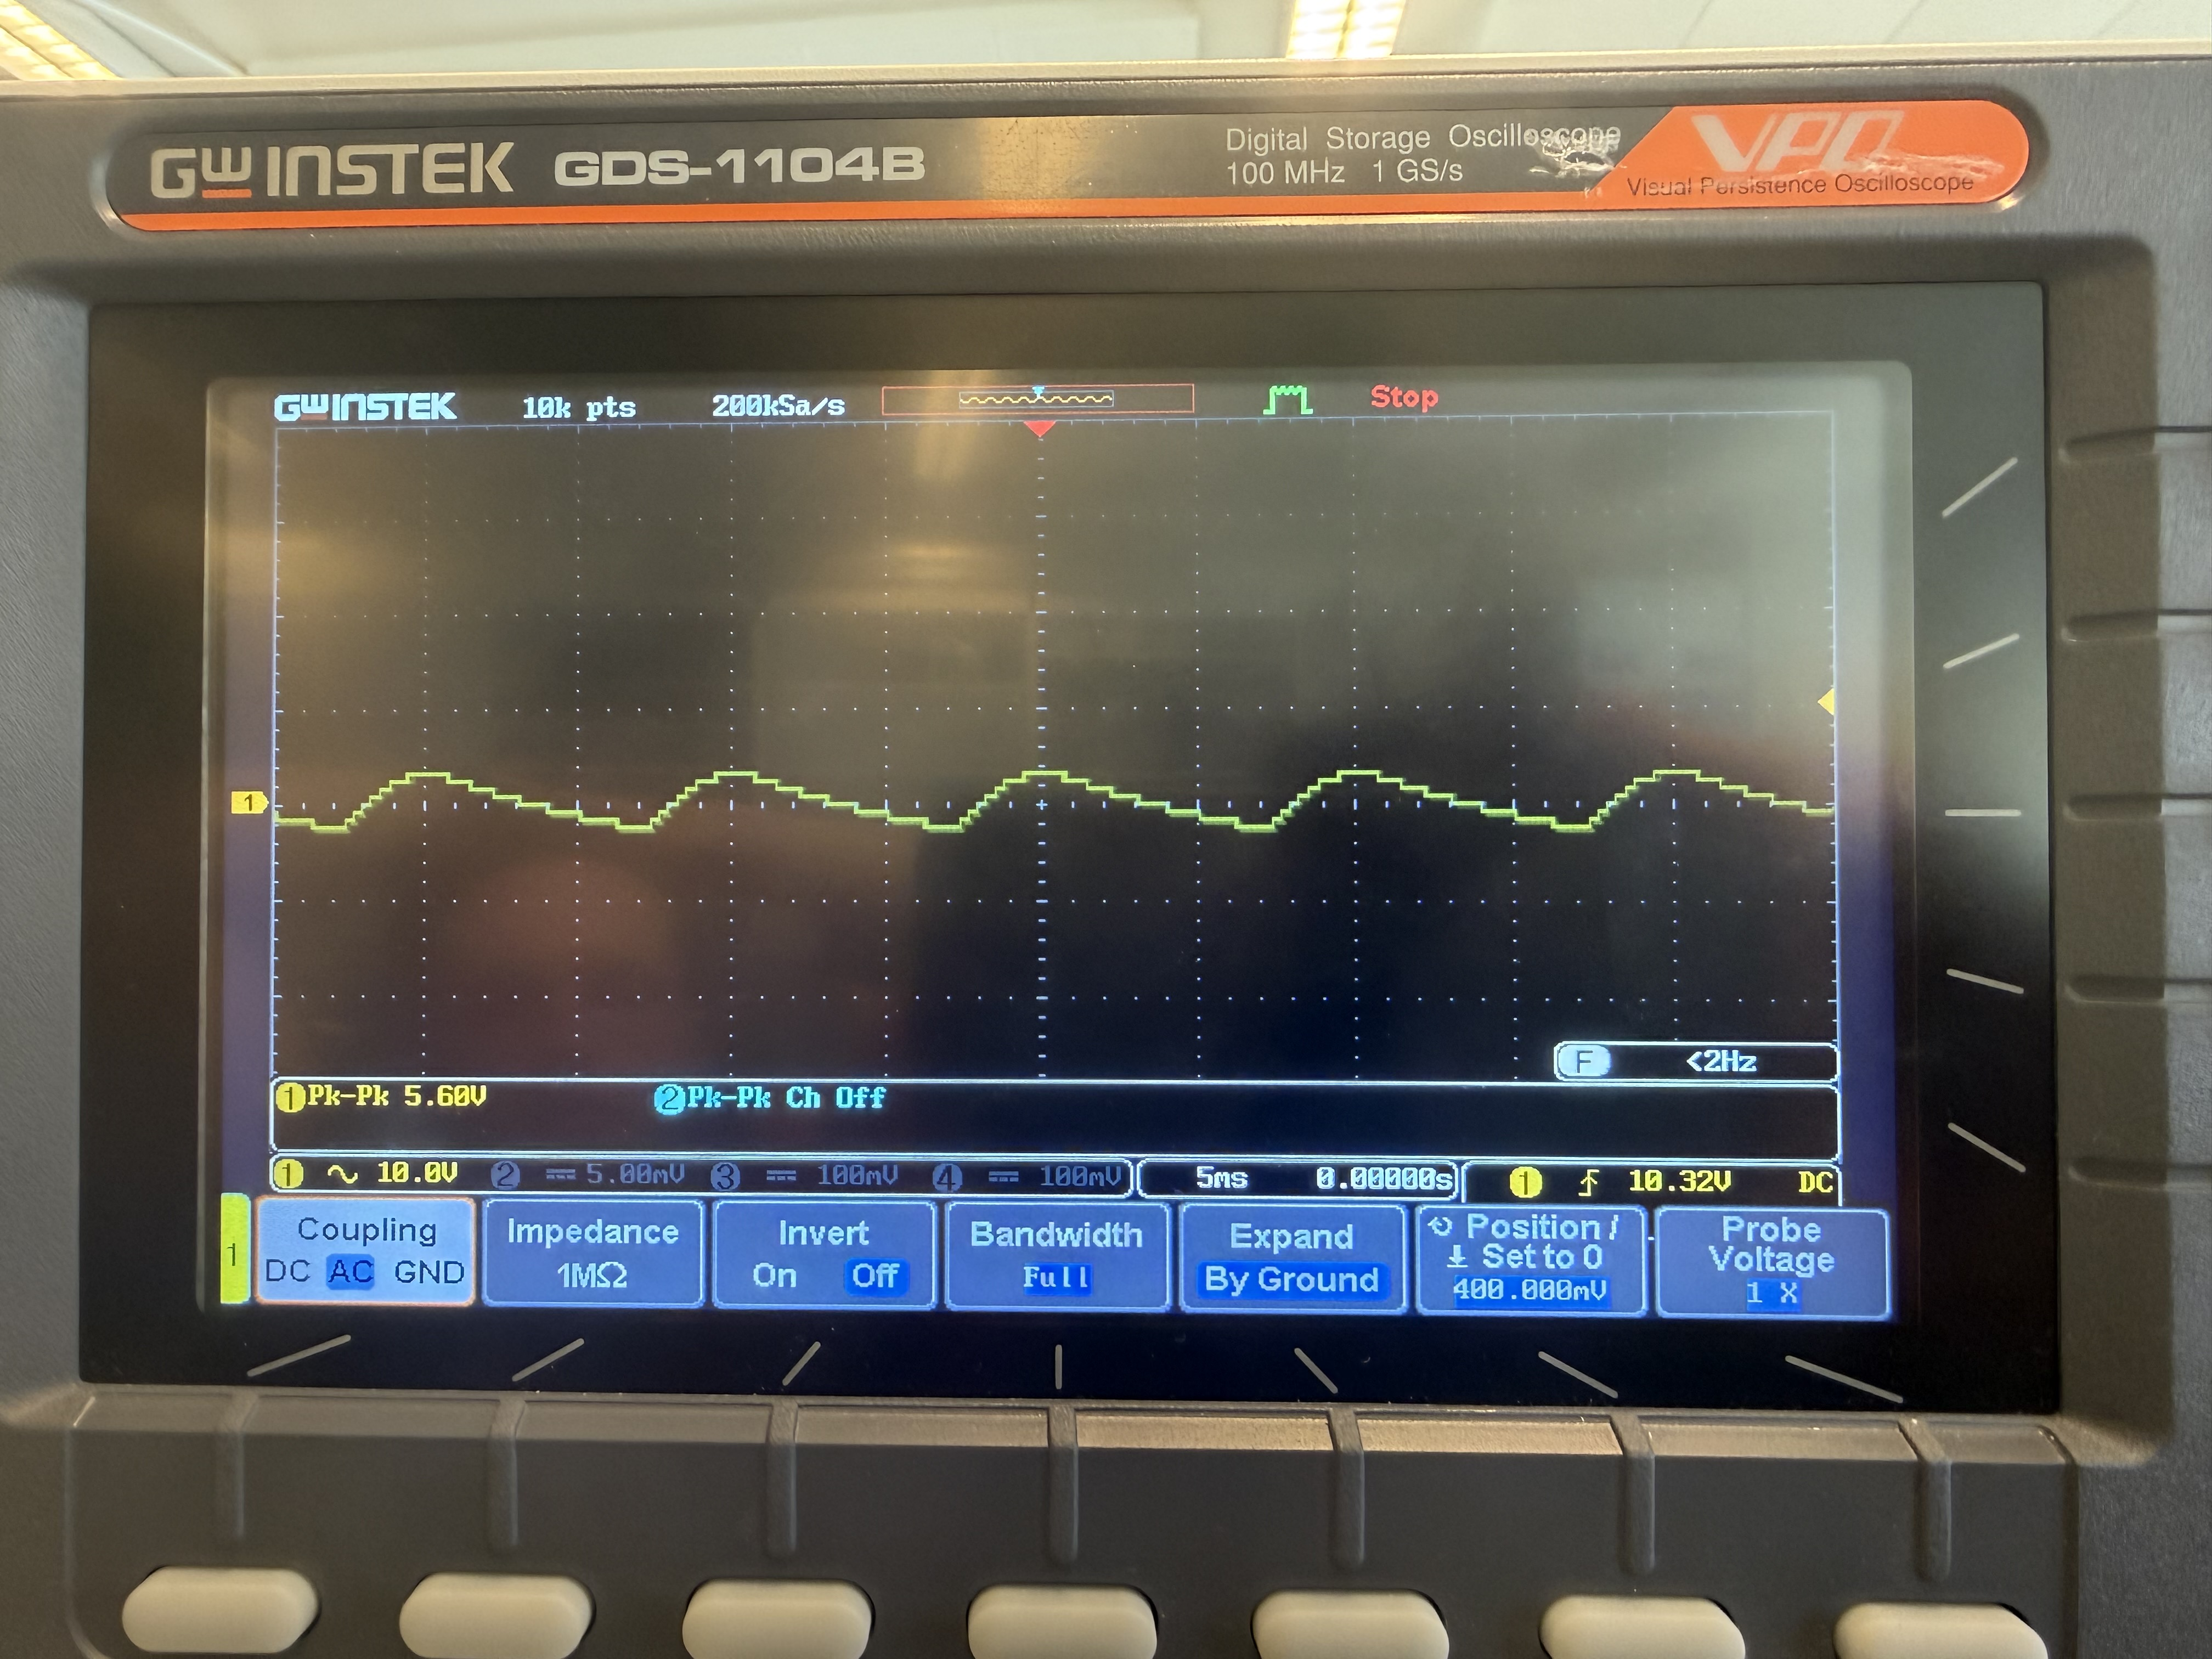
\includegraphics[width=0.7\textwidth]{Media/IMG_0875.jpeg}
                \caption{AC-mode: måling på spenningen over RC-leddet med $100\mu F$}
                \label{fig:toveis_likeretting_transformator_RC2}
            \end{figure}

            Studere ripple nærmere med AC-mode. Rippelens peak-peak-verdi kan leses av fra oscilloskopet, og er lik $Vpp=5.60V$.

    \subsubsection{RC-ledd: $C2 = 10\mu F$}
        \begin{figure}[H]
            \centering
            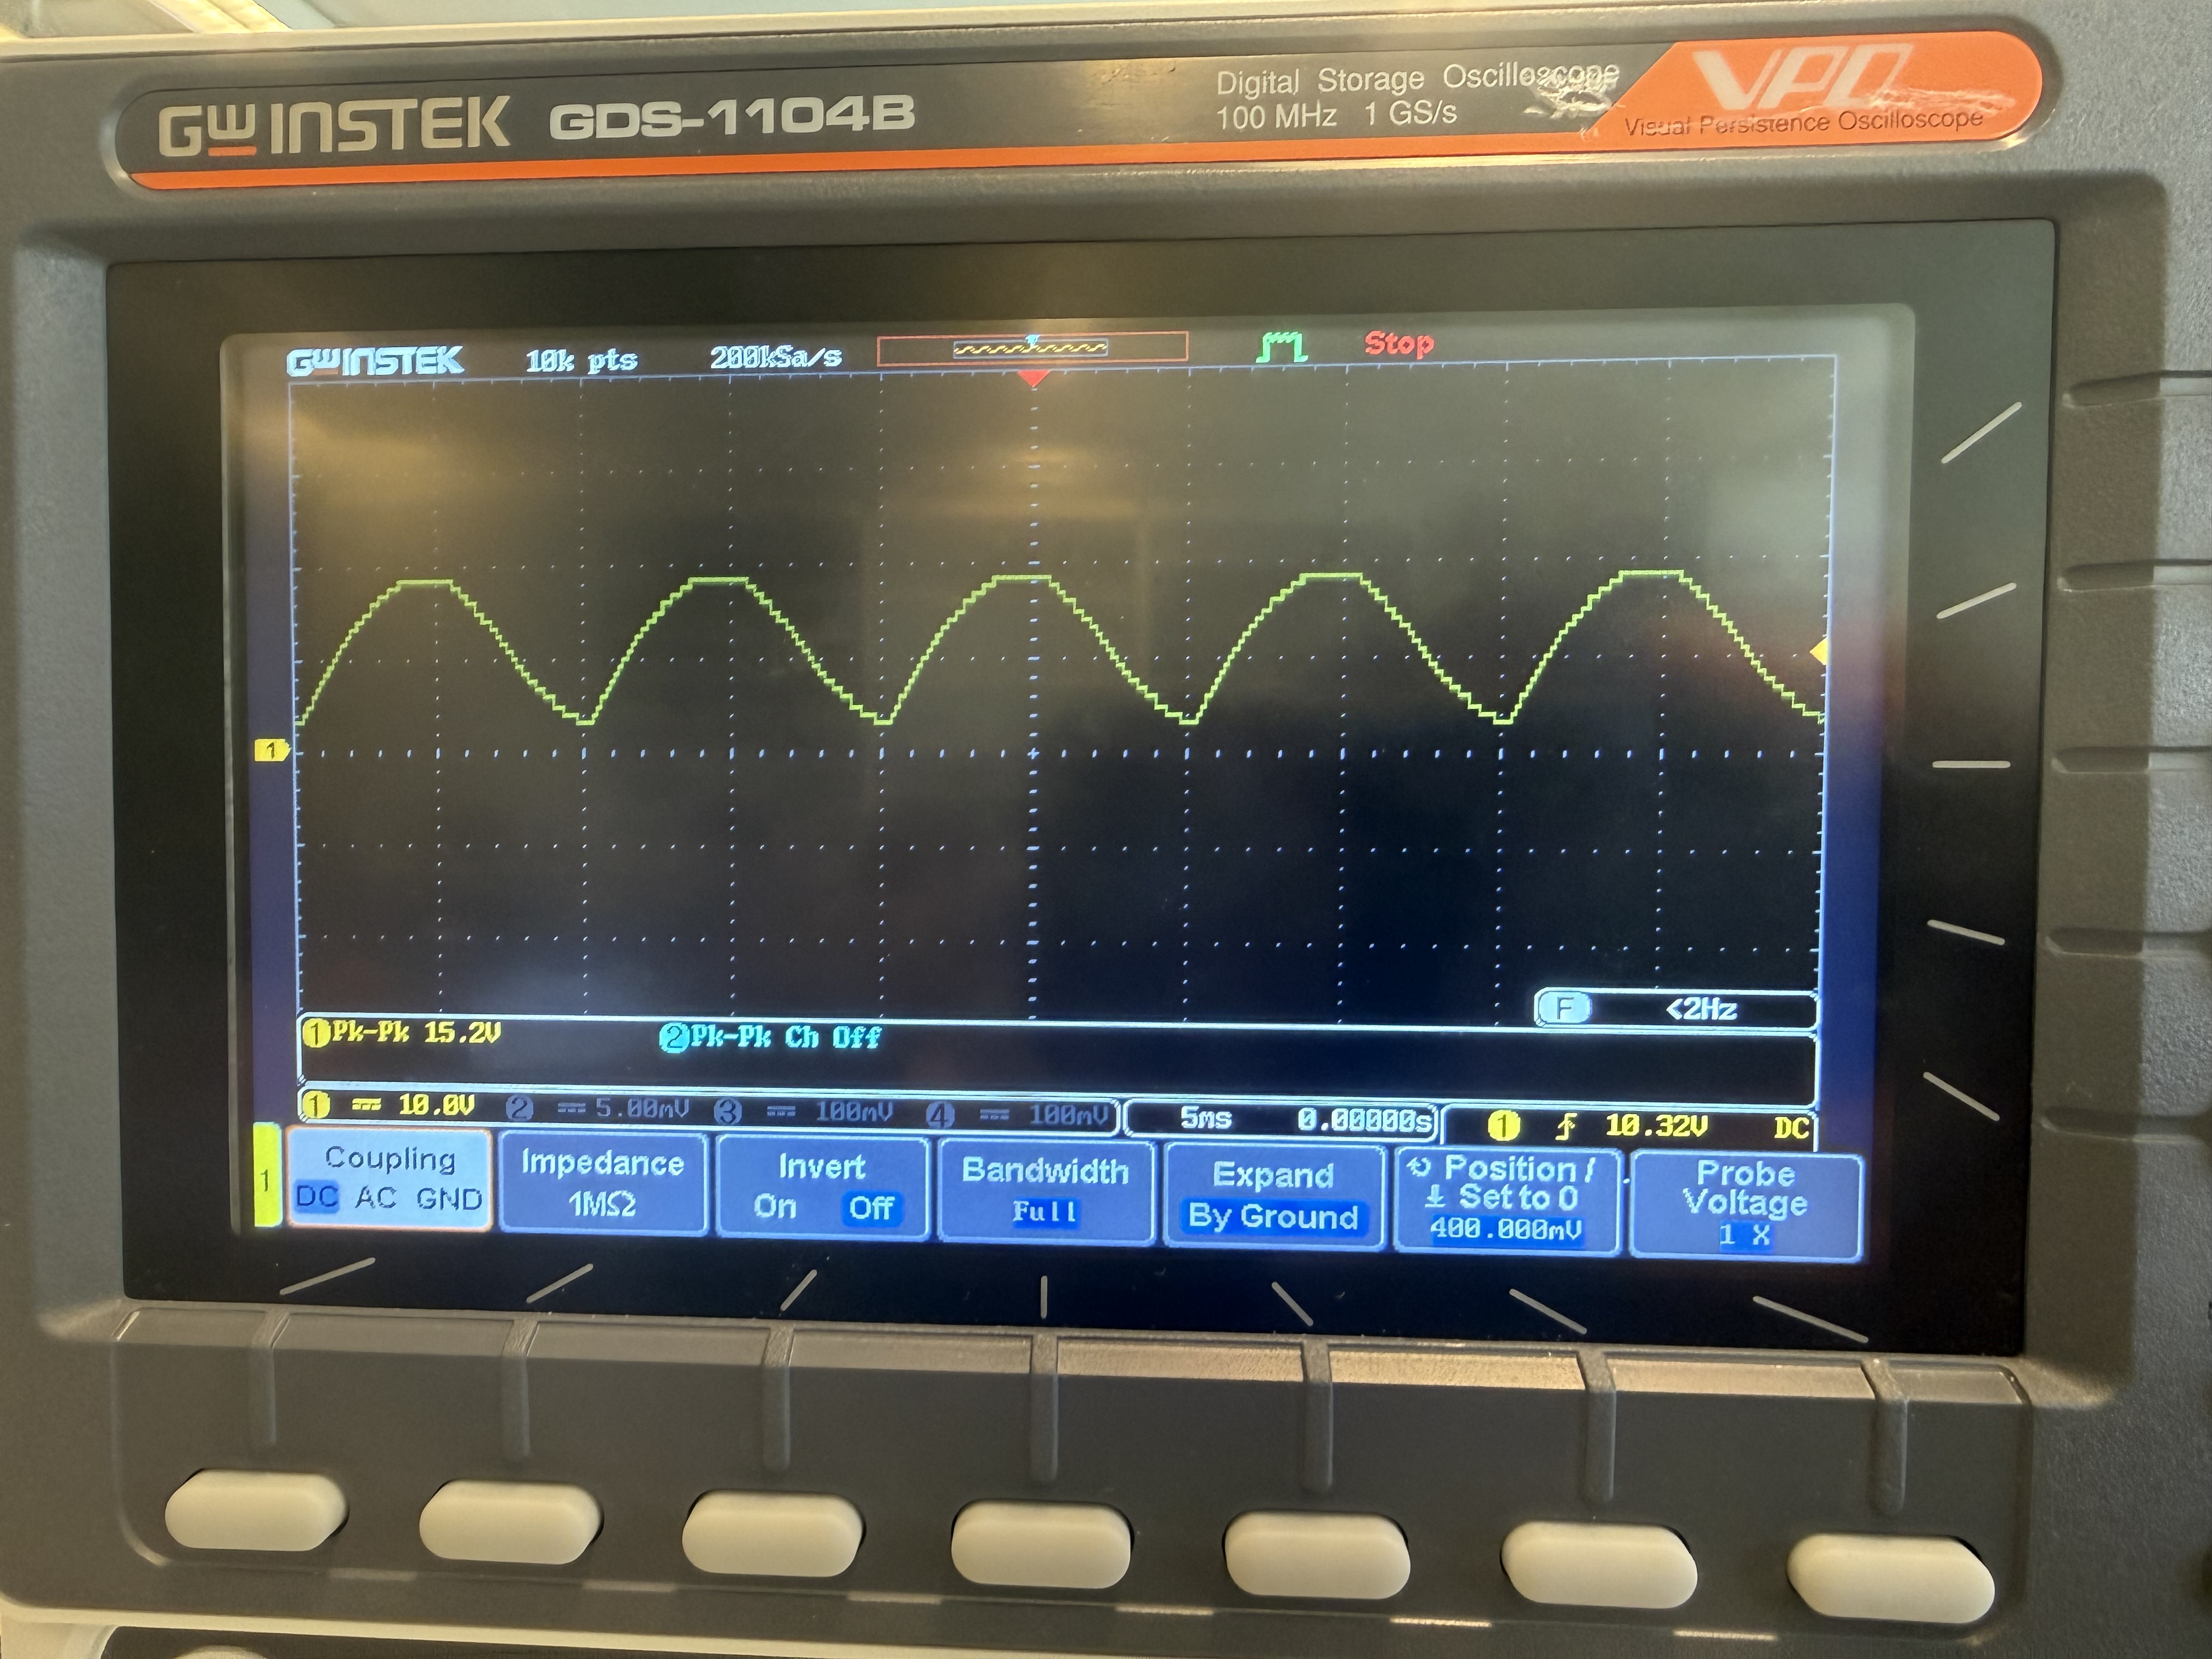
\includegraphics[width=0.7\textwidth]{Media/IMG_0876.jpeg}
            \caption{Måling på spenningen over RC-leddet med $10\mu F$}
            \label{fig:toveis_likeretting_transformator_RC3}
        \end{figure}
        